\documentclass[12pt,a4paper]{article}

% ─── Encodage & langue ───────────────────────────────────────────────────────
\usepackage[utf8]{inputenc}
\usepackage[T1]{fontenc}
\usepackage[french]{babel}

% ─── Mise en page ────────────────────────────────────────────────────────────
\usepackage[top=2.5cm, bottom=2.5cm, left=2.8cm, right=2.8cm]{geometry}
\usepackage{setspace}
\onehalfspacing

% ─── Polices & couleurs ──────────────────────────────────────────────────────
\usepackage{lmodern}
\usepackage{xcolor}
\definecolor{hadoopBlue}{HTML}{1A73E8}
\definecolor{codeGray}{HTML}{F5F5F5}
\definecolor{accentGreen}{HTML}{2E7D32}

% ─── Graphiques & figures ────────────────────────────────────────────────────
\usepackage{graphicx}
\graphicspath{{images_Rapport/}}
\usepackage{float}
\usepackage{subcaption}
\usepackage{caption}
\captionsetup{font=small, labelfont=bf}

% ─── Tableaux ────────────────────────────────────────────────────────────────
\usepackage{booktabs}
\usepackage{array}
\usepackage{tabularx}
\usepackage{multirow}
\usepackage{colortbl}

% ─── Code source ─────────────────────────────────────────────────────────────
\usepackage{listings}
\lstset{
  backgroundcolor=\color{codeGray},
  basicstyle=\ttfamily\small,
  breaklines=true,
  frame=single,
  rulecolor=\color{gray!40},
  showstringspaces=false,
  keywordstyle=\color{hadoopBlue}\bfseries,
  commentstyle=\color{gray},
  stringstyle=\color{accentGreen},
  numbers=left,
  numberstyle=\tiny\color{gray},
  numbersep=8pt,
}

% ─── Liens & PDF ─────────────────────────────────────────────────────────────
\usepackage[hidelinks]{hyperref}
\usepackage{url}

% ─── En-têtes / pieds de page ────────────────────────────────────────────────
\usepackage{fancyhdr}
\pagestyle{fancy}
\fancyhf{}
\fancyhead[L]{\small\textcolor{gray}{Projet Big Data — Hadoop MapReduce}}
\fancyhead[R]{\small\textcolor{gray}{\thepage}}
\renewcommand{\headrulewidth}{0.4pt}

% ─── Divers ──────────────────────────────────────────────────────────────────
\usepackage{amsmath}
\usepackage{enumitem}
\usepackage{tcolorbox}
\tcbuselibrary{skins}

% ─────────────────────────────────────────────────────────────────────────────
\begin{document}

% ═══════════════════════════════════════════════════════════════════════════════
%  PAGE DE TITRE
% ═══════════════════════════════════════════════════════════════════════════════
\begin{titlepage}
  \centering
  \vspace*{1.5cm}

  {\LARGE \textbf{Université — Filière Informatique / Big Data}}\\[0.4cm]
  {\large Année universitaire 2025--2026}

  \vspace{1.5cm}
  \rule{\linewidth}{1.5pt}\\[0.3cm]
  {\Huge \textbf{Projet Big Data}}\\[0.4cm]
  {\LARGE \textcolor{hadoopBlue}{\textbf{Analyse E-commerce à grande échelle\\
  avec Hadoop MapReduce}}}\\[0.3cm]
  \rule{\linewidth}{1.5pt}

  \vspace{1.5cm}

  \begin{tcolorbox}[colback=hadoopBlue!8, colframe=hadoopBlue, sharp corners,
                    width=0.85\textwidth]
    \centering
    \textbf{Technologies utilisées :}\\[0.3em]
    Apache Hadoop 3.2.1 \quad|\quad HDFS \quad|\quad YARN\\
    MapReduce (Java) \quad|\quad Docker \quad|\quad Python / Matplotlib
  \end{tcolorbox}

  \vspace{2cm}

  \begin{tabular}{ll}
    \textbf{Réalisé par :}  & Khalid Abfaraj \\[0.3em]
    \textbf{Encadrant :}    & [Nom de l'encadrant] \\[0.3em]
    \textbf{Date :}         & Juin 2026 \\
  \end{tabular}

  \vfill
\end{titlepage}

% ═══════════════════════════════════════════════════════════════════════════════
%  TABLE DES MATIÈRES
% ═══════════════════════════════════════════════════════════════════════════════
\tableofcontents
\newpage

% ═══════════════════════════════════════════════════════════════════════════════
%  1. INTRODUCTION
% ═══════════════════════════════════════════════════════════════════════════════
\section{Introduction}

\subsection{Contexte et motivation}

L'explosion du commerce électronique génère des volumes de données considérables :
transactions, évaluations clients, informations géographiques et temporelles.
Analyser ces données à l'aide d'outils traditionnels devient rapidement impossible
dès que le volume dépasse quelques centaines de millions de lignes.

Ce projet s'inscrit dans le cadre du cours de \textit{Big Data} et vise à mettre
en œuvre un pipeline complet de traitement distribué, depuis la génération d'un
jeu de données synthétique jusqu'à la visualisation des résultats, en passant par
l'exécution de jobs \textbf{MapReduce} sur un cluster \textbf{Hadoop} conteneurisé.

\subsection{Objectifs}

\begin{enumerate}[leftmargin=*]
  \item Déployer un cluster Hadoop multi-nœuds via Docker Compose.
  \item Générer un dataset e-commerce synthétique réaliste de \textbf{20 millions
        de lignes} ($\approx$1,8 Go).
  \item Concevoir et exécuter \textbf{quatre jobs MapReduce} en Java sur YARN.
  \item Visualiser les résultats sous forme de dashboard graphique.
\end{enumerate}

\subsection{Plan du rapport}

Le rapport est organisé comme suit : la section~\ref{sec:archi} présente
l'architecture technique du cluster ; la section~\ref{sec:dataset} décrit la
génération du jeu de données ; la section~\ref{sec:mapreduce} détaille les quatre
jobs MapReduce ; la section~\ref{sec:resultats} analyse les résultats obtenus ;
la section~\ref{sec:visu} présente la visualisation ; enfin la
section~\ref{sec:conclusion} conclut le rapport.

% ═══════════════════════════════════════════════════════════════════════════════
%  2. ARCHITECTURE DU CLUSTER
% ═══════════════════════════════════════════════════════════════════════════════
\section{Architecture du cluster Hadoop}
\label{sec:archi}

\subsection{Infrastructure Docker}

Le cluster est entièrement conteneurisé avec \textbf{Docker Compose}, ce qui
permet de simuler un environnement distribué sur une seule machine de
développement. L'image de base utilisée est
\texttt{bde2020/hadoop-namenode:2.0.0-hadoop3.2.1-java8}.

Le fichier \texttt{docker-compose.yml} définit \textbf{7 services} :

\begin{table}[H]
  \centering
  \caption{Services du cluster Hadoop}
  \label{tab:services}
  \begin{tabularx}{\textwidth}{lXl}
    \toprule
    \textbf{Service} & \textbf{Rôle} & \textbf{Port exposé} \\
    \midrule
    \texttt{namenode}        & Gestion des métadonnées HDFS, point d'entrée & 9870, 9000 \\
    \texttt{datanode1}       & Stockage des blocs HDFS (réplique 1)         & ---        \\
    \texttt{datanode2}       & Stockage des blocs HDFS (réplique 2)         & ---        \\
    \texttt{datanode3}       & Stockage des blocs HDFS (réplique 3)         & ---        \\
    \texttt{resourcemanager} & Ordonnancement des jobs YARN                 & 8088       \\
    \texttt{nodemanager}     & Exécution des conteneurs YARN                & ---        \\
    \texttt{historyserver}   & Historique des jobs MapReduce terminés       & 8188       \\
    \bottomrule
  \end{tabularx}
\end{table}

\subsection{État du cluster — docker ps}

La figure~\ref{fig:docker_ps} montre les 7 conteneurs Hadoop en cours d'exécution,
tous avec le statut \texttt{Up (healthy)}, confirmant que le cluster est
opérationnel.

\begin{figure}[H]
  \centering
  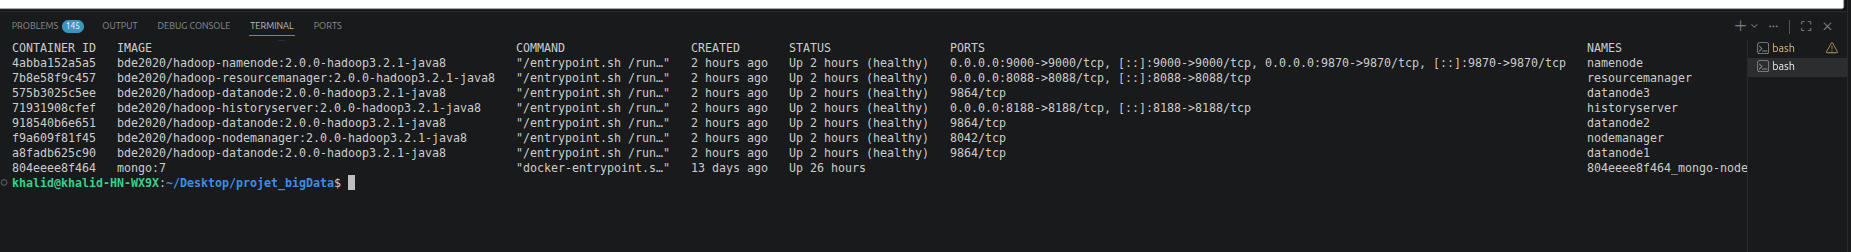
\includegraphics[width=\textwidth]{docker_ps.png}
  \caption{Sortie de \texttt{docker ps} — les 7 conteneurs Hadoop sont actifs et sains}
  \label{fig:docker_ps}
\end{figure}

\subsection{Configuration HDFS}

La réplication des blocs est fixée à \textbf{3} (valeur par défaut Hadoop),
assurée par les trois DataNodes. La compression \textbf{Snappy} est activée.

\begin{lstlisting}[language=bash, caption={Extrait de hadoop.env — configuration HDFS/YARN}]
HDFS_CONF_dfs_replication=3
HDFS_CONF_dfs_webhdfs_enabled=true
CORE_CONF_io_compression_codecs=org.apache.hadoop.io.compress.SnappyCodec
MAPRED_CONF_mapreduce_framework_name=yarn
\end{lstlisting}

\subsection{Interface web du NameNode}

L'interface web HDFS (\texttt{localhost:9870}) permet de superviser l'état du
cluster, les DataNodes et l'espace de stockage disponible.

\begin{figure}[H]
  \centering
  \begin{subfigure}{0.48\textwidth}
    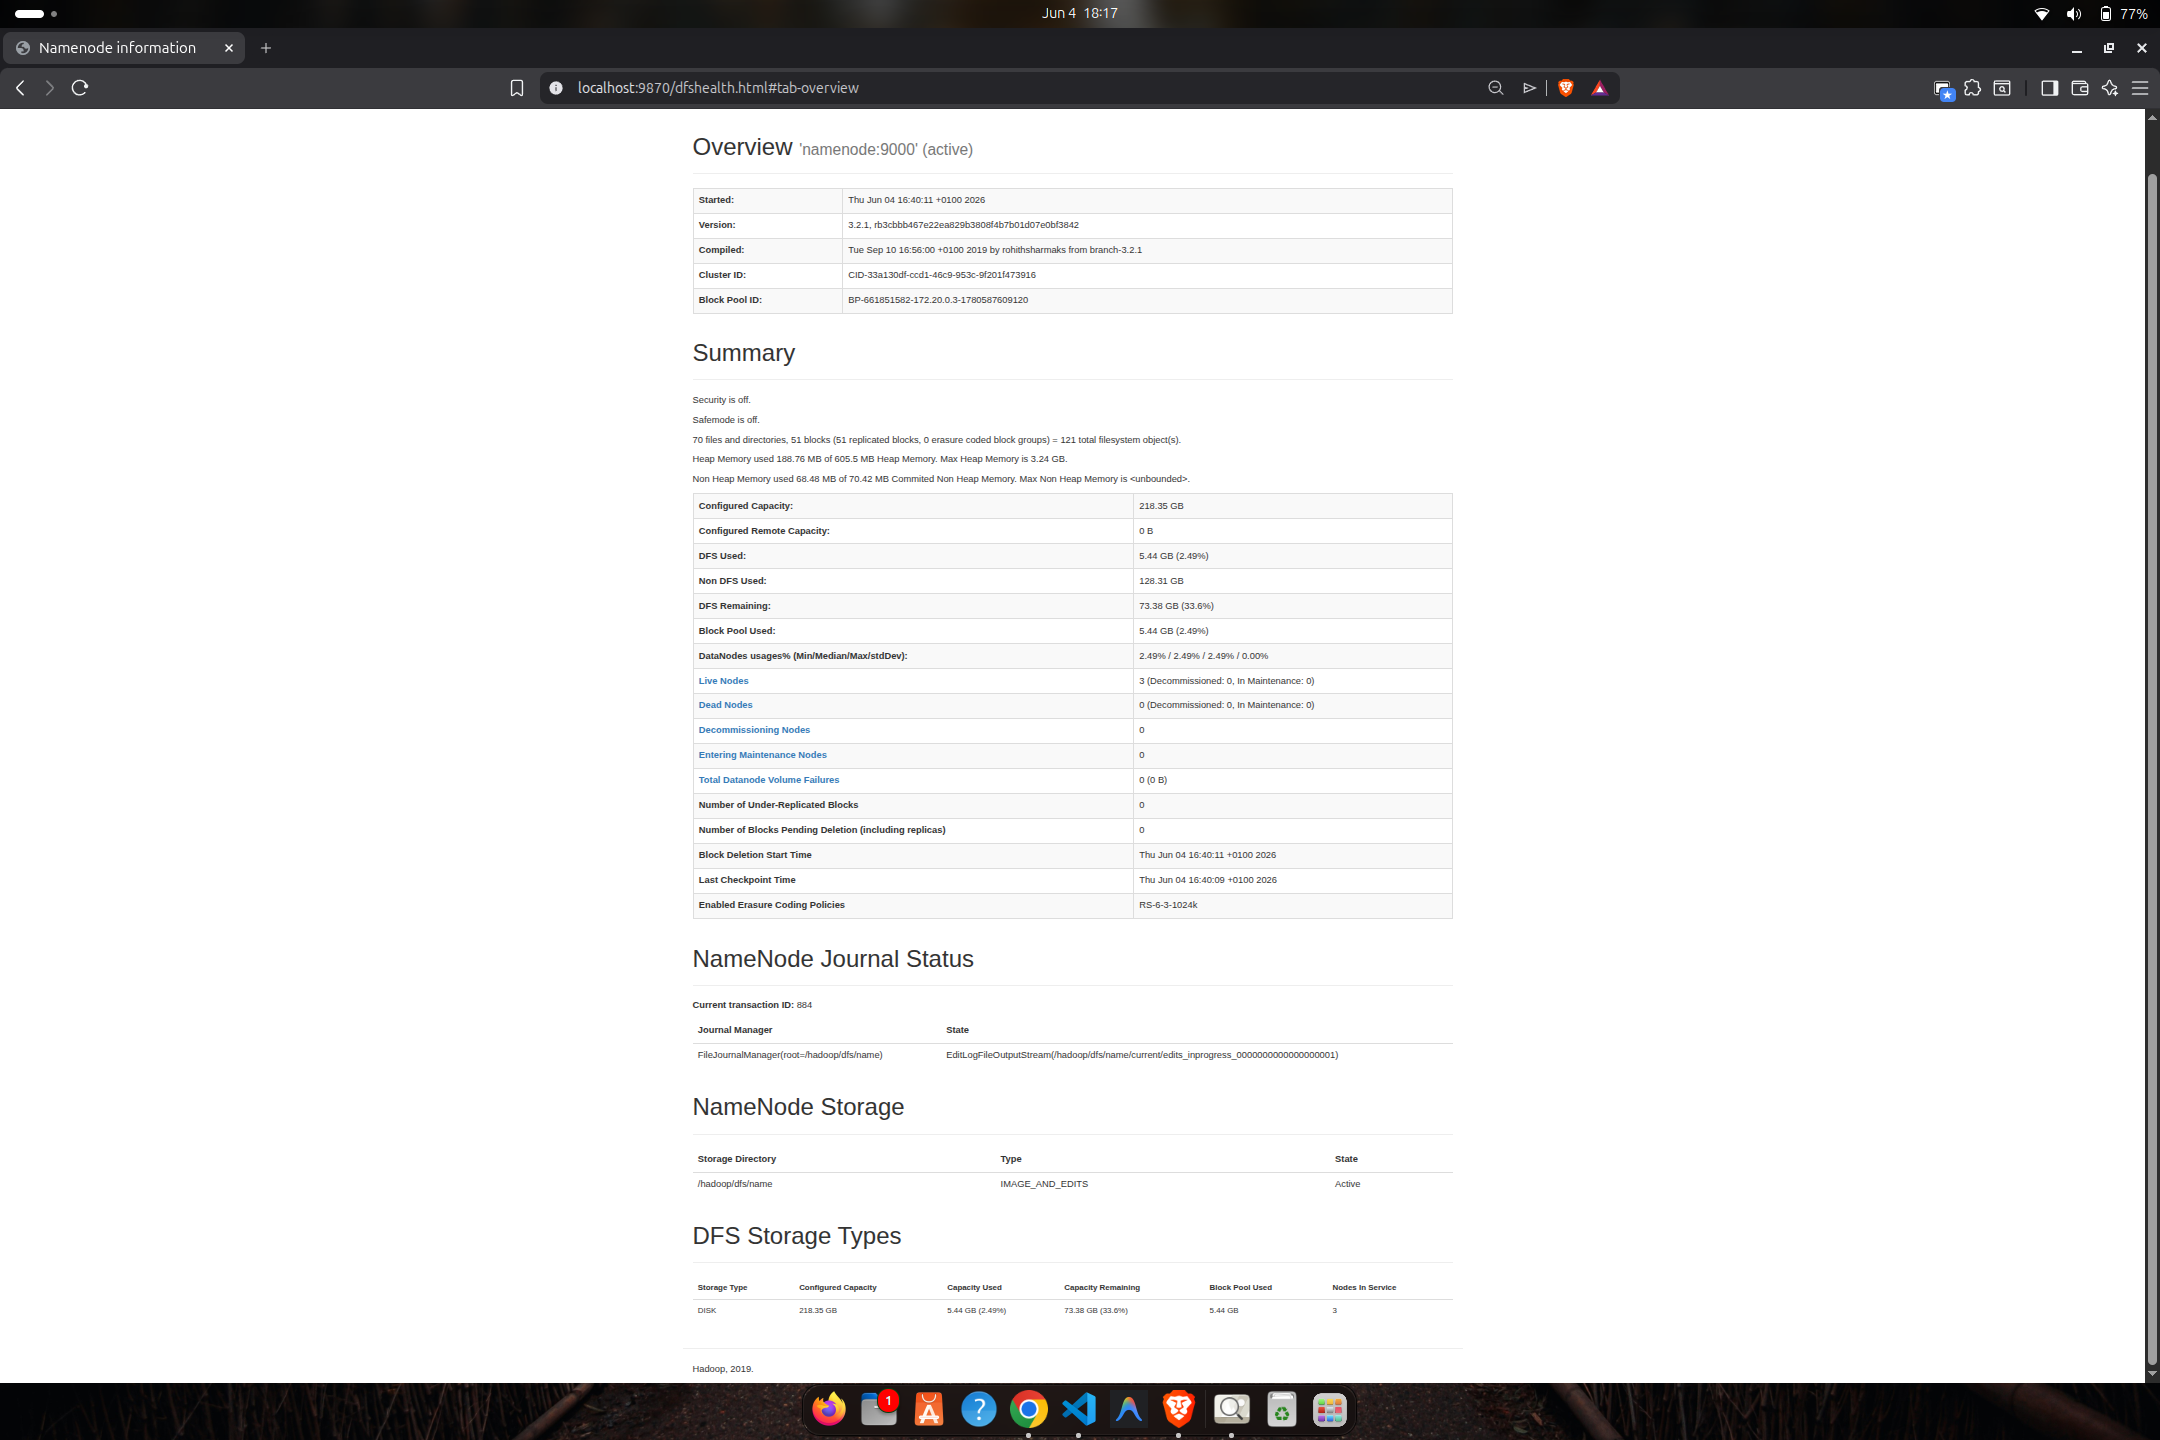
\includegraphics[width=\textwidth]{namenode_overview.png}
    \caption{Vue d'ensemble — NameNode Overview}
    \label{fig:namenode_overview}
  \end{subfigure}
  \hfill
  \begin{subfigure}{0.48\textwidth}
    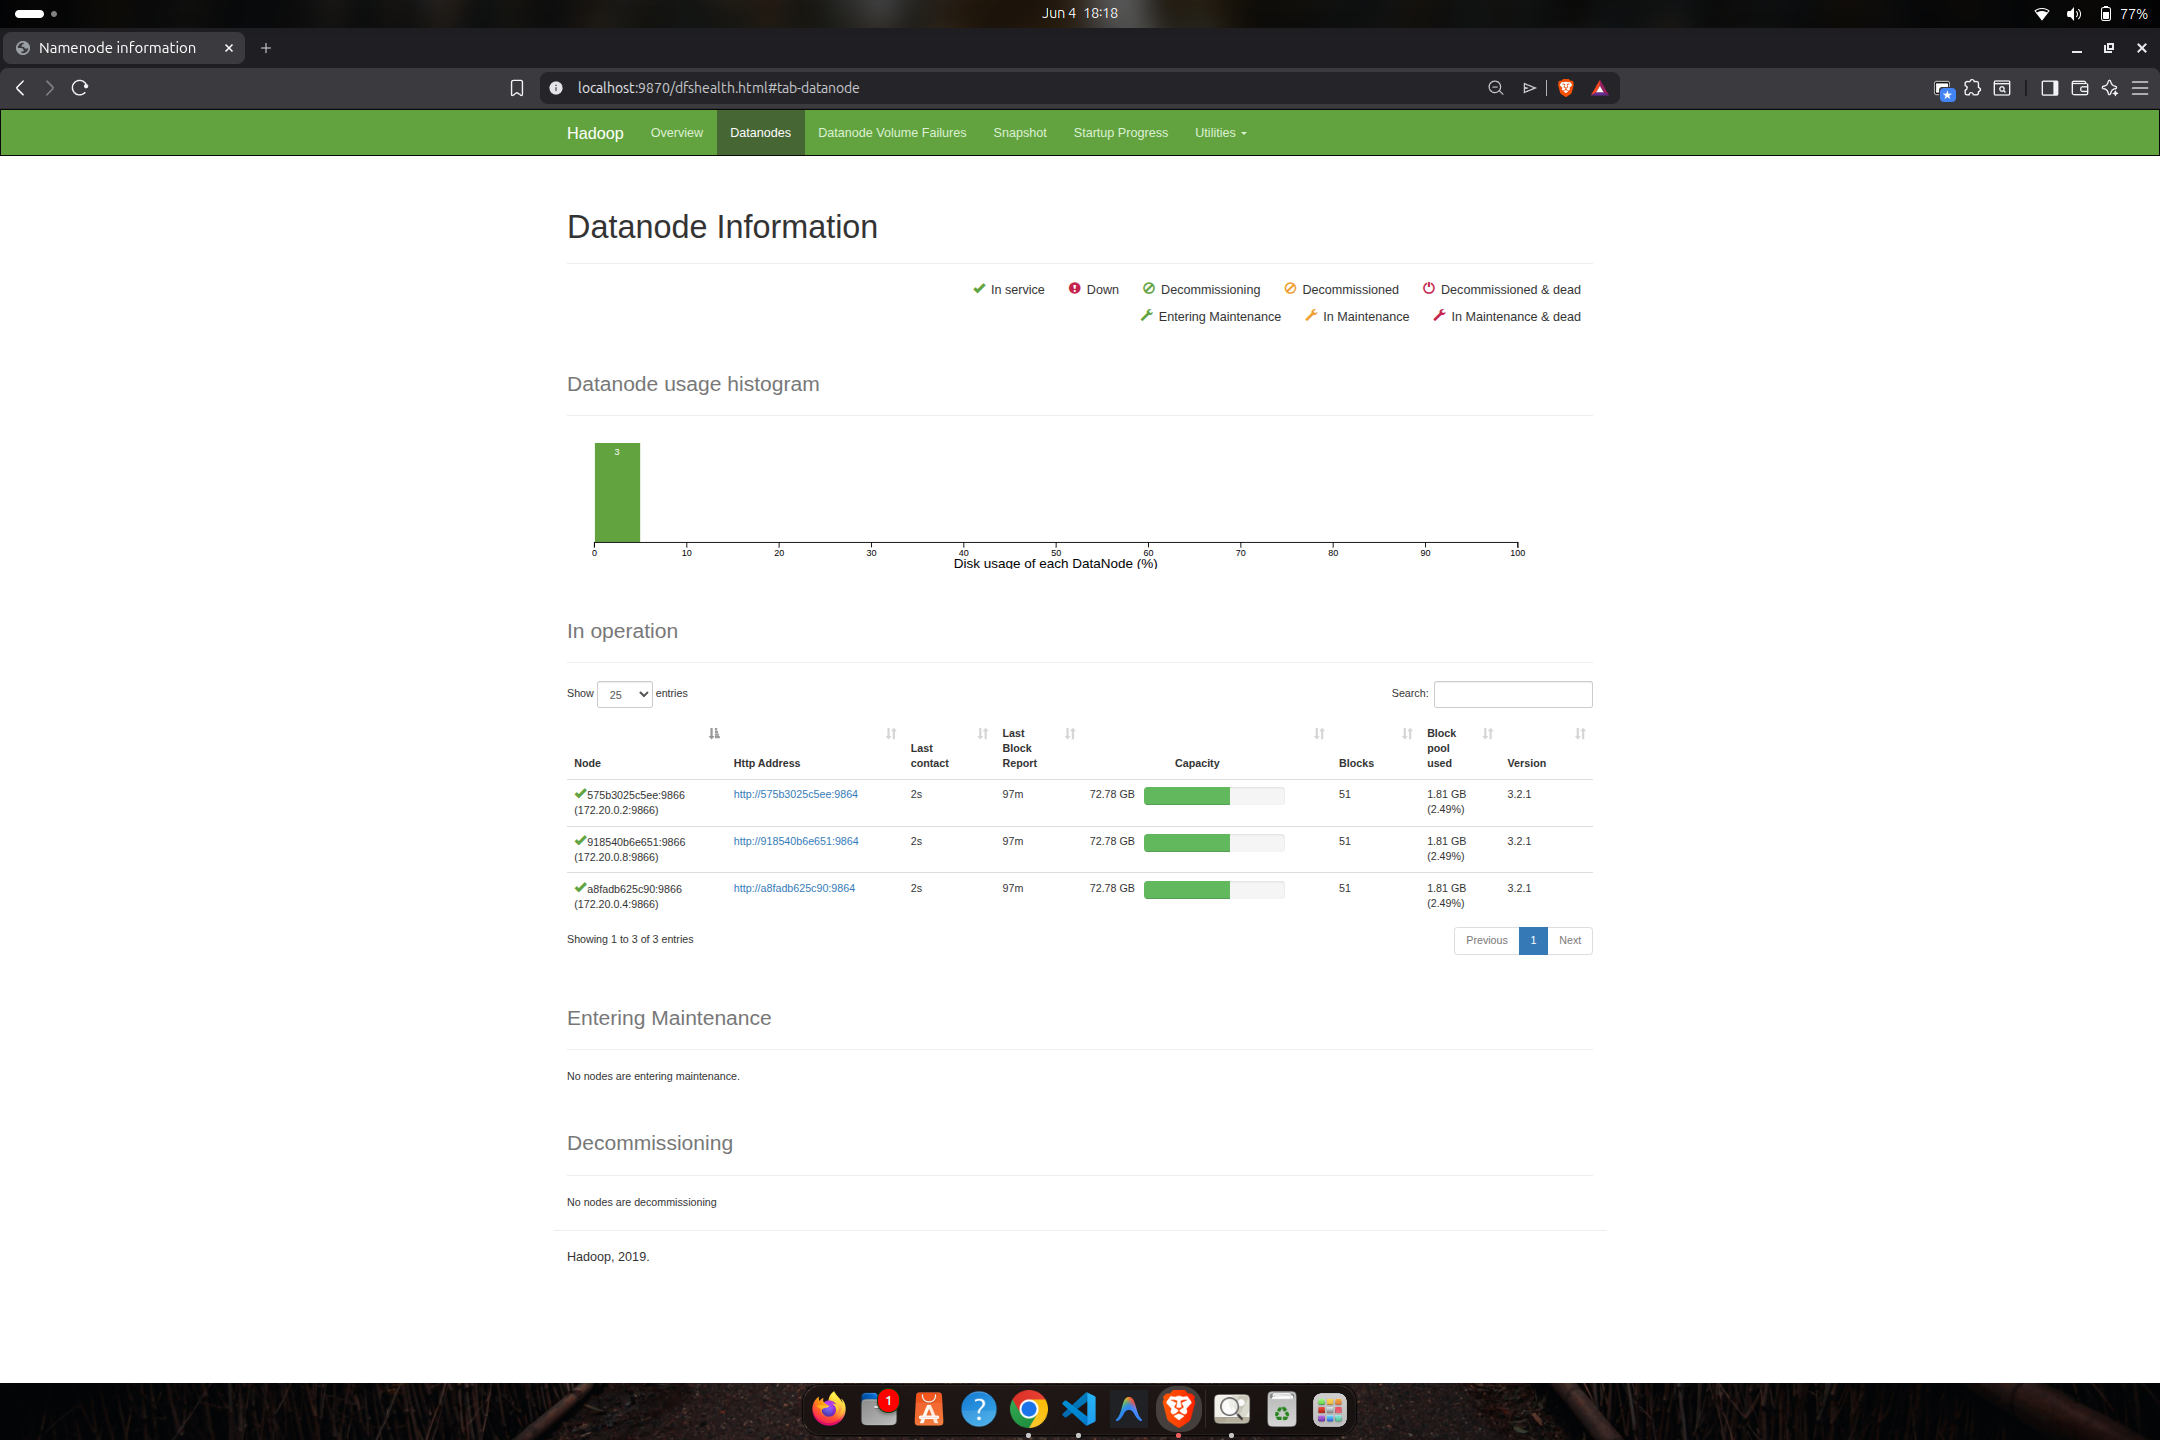
\includegraphics[width=\textwidth]{datanodes.png}
    \caption{Datanode Information — 3 nœuds actifs}
    \label{fig:datanodes}
  \end{subfigure}
  \caption{Interface web Hadoop NameNode (\texttt{localhost:9870})}
  \label{fig:namenode_ui}
\end{figure}

% ═══════════════════════════════════════════════════════════════════════════════
%  3. GÉNÉRATION ET CHARGEMENT DU DATASET
% ═══════════════════════════════════════════════════════════════════════════════
\section{Génération et chargement du jeu de données}
\label{sec:dataset}

\subsection{Description du dataset}

Le jeu de données est généré par le script Python \texttt{generate\_dataset.py}.
Il simule des commandes e-commerce pour un marché français sur la période
\textbf{janvier 2020 -- décembre 2023}.

\begin{table}[H]
  \centering
  \caption{Structure du fichier CSV \texttt{ecommerce\_data.csv}}
  \label{tab:schema}
  \begin{tabularx}{\textwidth}{llX}
    \toprule
    \textbf{Colonne} & \textbf{Type} & \textbf{Description} \\
    \midrule
    \texttt{order\_id}         & String  & Identifiant unique de commande (\texttt{ORDxxxxxxxxx}) \\
    \texttt{customer\_id}      & String  & Identifiant client (\texttt{CUSTxxxxxx}, 500\,000 clients) \\
    \texttt{product\_id}       & String  & Identifiant produit (\texttt{PRODxxxxx}, 10\,000 produits) \\
    \texttt{category}          & String  & Catégorie parmi 10 (électronique, vêtements, livres\ldots) \\
    \texttt{seller\_region}    & String  & Région du vendeur (10 régions françaises) \\
    \texttt{customer\_region}  & String  & Région du client (10 régions françaises) \\
    \texttt{price}             & Float   & Prix du produit (variable selon la catégorie) \\
    \texttt{freight\_value}    & Float   & Frais de livraison (5--20\% du prix) \\
    \texttt{review\_score}     & Integer & Note client de 1 à 5 étoiles \\
    \texttt{order\_date}       & String  & Mois de la commande (format \texttt{YYYY-MM}) \\
    \bottomrule
  \end{tabularx}
\end{table}

\subsection{Paramètres de génération}

\begin{table}[H]
  \centering
  \caption{Caractéristiques du dataset généré}
  \label{tab:dataset_stats}
  \begin{tabular}{ll}
    \toprule
    \textbf{Paramètre} & \textbf{Valeur} \\
    \midrule
    Nombre de lignes   & 20\,000\,000 \\
    Taille sur disque  & 1,8 Go \\
    Période couverte   & Janvier 2020 -- Décembre 2023 (48 mois) \\
    Catégories         & 10 \\
    Régions            & 10 (régions françaises) \\
    Clients uniques    & 500\,000 \\
    Produits uniques   & 10\,000 \\
    \bottomrule
  \end{tabular}
\end{table}

\subsection{Fourchettes de prix par catégorie}

\begin{table}[H]
  \centering
  \caption{Plages de prix par catégorie}
  \label{tab:prix}
  \begin{tabular}{lcc}
    \toprule
    \textbf{Catégorie} & \textbf{Prix min (€)} & \textbf{Prix max (€)} \\
    \midrule
    Électronique    & 50    & 2\,000 \\
    Automobile      & 30    & 1\,500 \\
    Maison/Jardin   & 10    & 800    \\
    Sport           & 20    & 500    \\
    Vêtements       & 15    & 300    \\
    Jouets          & 10    & 200    \\
    Santé           & 5     & 200    \\
    Beauté          & 5     & 150    \\
    Alimentation    & 3     & 100    \\
    Livres          & 8     & 80     \\
    \bottomrule
  \end{tabular}
\end{table}

\subsection{Pipeline d'exécution — étapes 1 à 3}

Le script \texttt{run\_ecommerce.sh} orchestre tout le pipeline. La
figure~\ref{fig:script_etapes} montre les trois premières étapes : vérification
du dataset (1,8 Go déjà présent), copie vers le conteneur NameNode
(1,92 GB transféré), puis chargement dans HDFS avec vérification.

\begin{figure}[H]
  \centering
  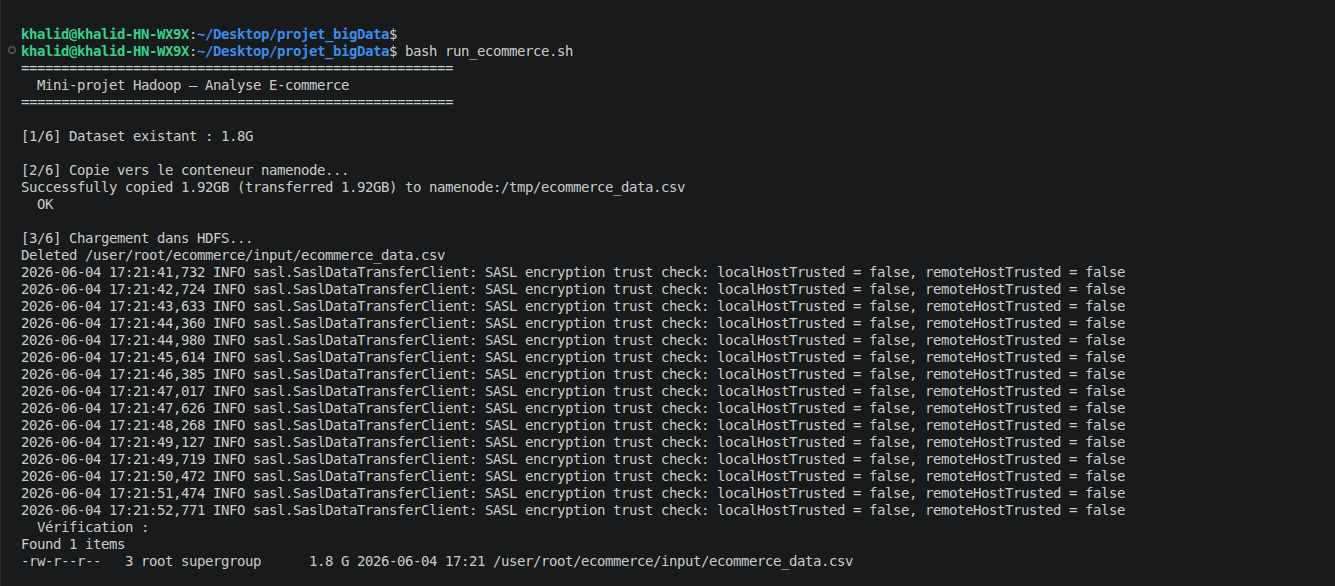
\includegraphics[width=\textwidth]{script_etape1_3.png}
  \caption{Exécution du script — étapes 1/6 (dataset), 2/6 (copie Docker) et 3/6 (upload HDFS)}
  \label{fig:script_etapes}
\end{figure}

\subsection{Structure HDFS}

Le fichier est chargé sous le chemin \texttt{/user/root/ecommerce/input/}.
L'interface \textit{Browse Directory} de HDFS (figure~\ref{fig:hdfs_browse})
confirme la présence du répertoire \texttt{ecommerce}.

\begin{figure}[H]
  \centering
  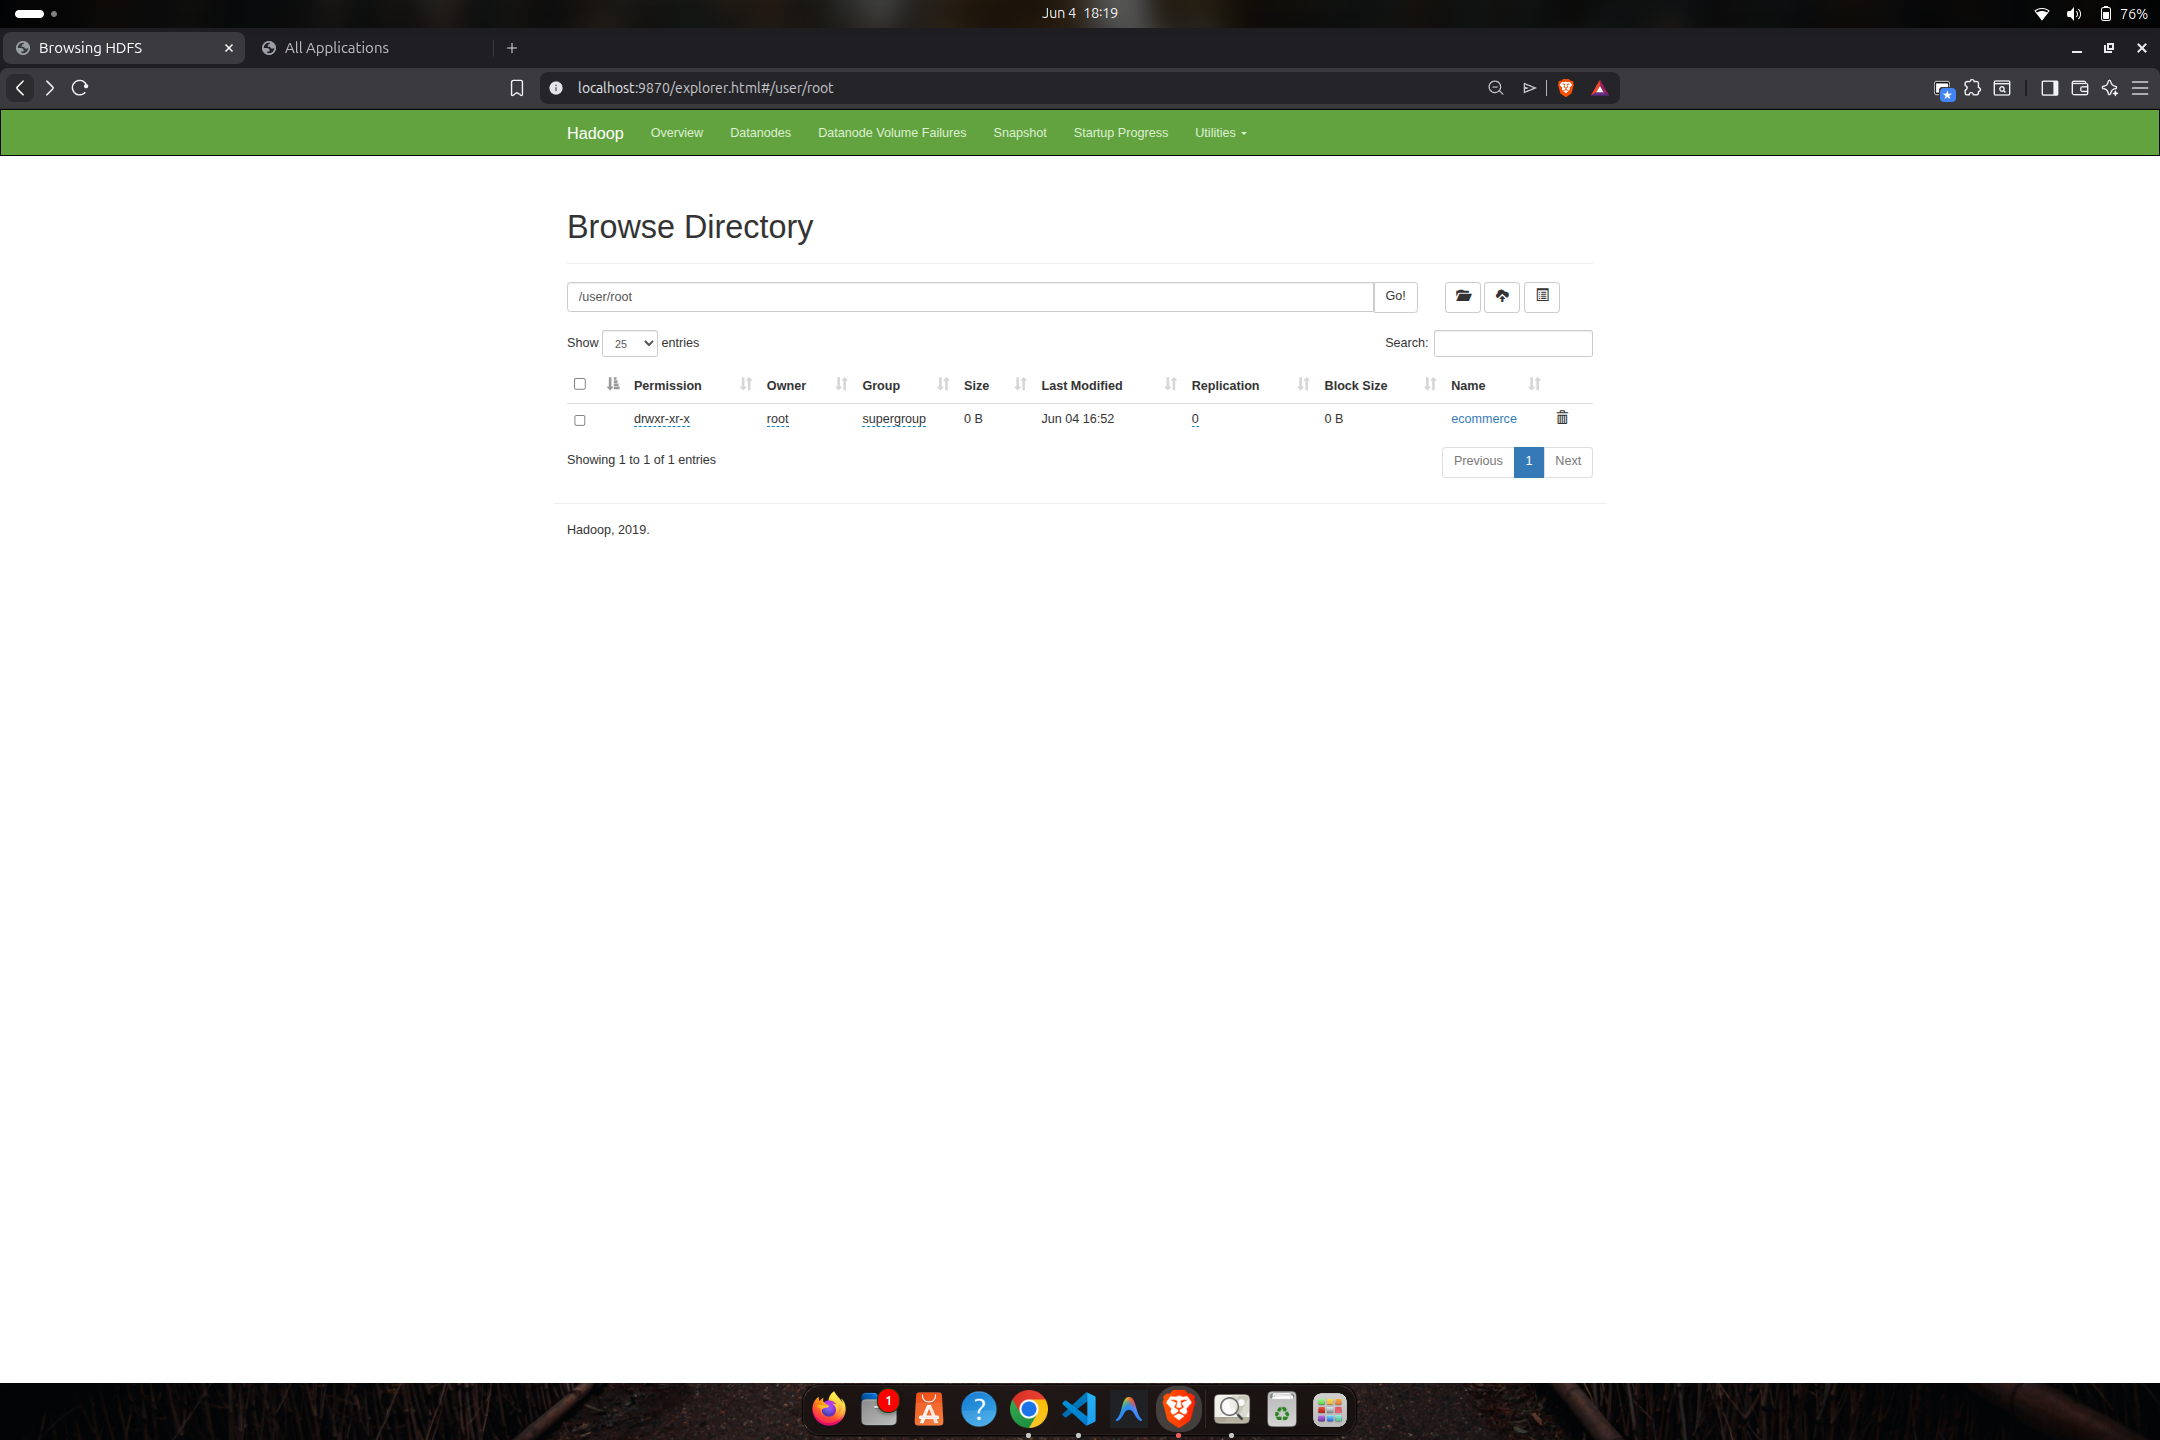
\includegraphics[width=0.85\textwidth]{hdfs_browse.png}
  \caption{HDFS Browse Directory — répertoire \texttt{/user/root} contenant le dossier \texttt{ecommerce}}
  \label{fig:hdfs_browse}
\end{figure}

% ═══════════════════════════════════════════════════════════════════════════════
%  4. JOBS MAPREDUCE
% ═══════════════════════════════════════════════════════════════════════════════
\section{Jobs MapReduce}
\label{sec:mapreduce}

\subsection{Présentation générale}

Le fichier \texttt{EcommerceAnalysis.java} implémente quatre jobs MapReduce
indépendants dans une seule classe Java. Chaque job est sélectionné au moment
de l'exécution via un argument en ligne de commande :

\begin{lstlisting}[language=bash, caption={Invocation d'un job MapReduce}]
hadoop jar ecommerce.jar EcommerceAnalysis <job> <input> <output>
# jobs disponibles :
#   revenue_category | orders_region | ratings | monthly_trend
\end{lstlisting}

Tous les jobs partagent le même schéma d'entrée (CSV à 10 colonnes) et ignorent
la ligne d'en-tête via la condition \texttt{if (line.startsWith("order\_id"))}.

\subsection{Job 1 — Chiffre d'affaires par catégorie}

\textbf{Objectif :} calculer la somme des prix pour chaque catégorie de produit.

\begin{description}[leftmargin=2em]
  \item[Mapper] Émet \texttt{(catégorie, prix)} pour chaque ligne valide.
  \item[Combiner] Pré-agrège localement les prix par catégorie.
  \item[Reducer] Additionne tous les prix reçus pour chaque catégorie.
  \item[Types de sortie] \texttt{Text} $\rightarrow$ \texttt{DoubleWritable}
\end{description}

\begin{lstlisting}[language=java, caption={Mapper — Chiffre d'affaires par catégorie}]
public void map(Object key, Text value, Context ctx)
        throws IOException, InterruptedException {
    String line = value.toString();
    if (line.startsWith("order_id")) return;
    String[] f = line.split(",");
    if (f.length <= COL_PRICE) return;
    try {
        category.set(f[COL_CATEGORY].trim());
        price.set(Double.parseDouble(f[COL_PRICE].trim()));
        ctx.write(category, price);
    } catch (NumberFormatException ignored) {}
}
\end{lstlisting}

\subsection{Job 2 — Nombre de commandes par région}

\textbf{Objectif :} compter le nombre de commandes par région cliente.

\begin{description}[leftmargin=2em]
  \item[Mapper] Émet \texttt{(région\_client, 1)} pour chaque commande.
  \item[Combiner] Compte local par région.
  \item[Reducer] Additionne les comptes de tous les mappers.
  \item[Types de sortie] \texttt{Text} $\rightarrow$ \texttt{IntWritable}
\end{description}

Ce job implémente le patron classique \textbf{Word Count} appliqué aux régions,
avec \texttt{ONE = new IntWritable(1)} pré-instancié pour éviter la pression GC.

\subsection{Job 3 — Distribution des notes clients}

\textbf{Objectif :} établir l'histogramme des évaluations (de 1 à 5 étoiles).

\begin{description}[leftmargin=2em]
  \item[Mapper] Émet \texttt{(note, 1)} pour chaque commande évaluée.
  \item[Reducer] Additionne les comptes par note.
  \item[Types de sortie] \texttt{IntWritable} $\rightarrow$ \texttt{IntWritable}
\end{description}

\subsection{Job 4 — Tendance mensuelle du chiffre d'affaires}

\textbf{Objectif :} calculer le CA agrégé pour chaque mois (2020--2023).

\begin{description}[leftmargin=2em]
  \item[Mapper] Émet \texttt{(mois, prix)} pour chaque commande (clé : \texttt{YYYY-MM}).
  \item[Reducer] Somme globale par mois.
  \item[Types de sortie] \texttt{Text} $\rightarrow$ \texttt{DoubleWritable}
\end{description}

Grâce au format \texttt{YYYY-MM}, le tri alphabétique de Hadoop garantit
automatiquement un tri chronologique dans la sortie.

\subsection{Optimisation : Combiner}

Tous les quatre jobs utilisent le \textbf{Combiner} identique au Reducer.
Il effectue une pré-agrégation locale sur chaque nœud avant le shuffle,
réduisant significativement le trafic réseau.

\begin{lstlisting}[language=java, caption={Configuration d'un job avec Combiner (exemple Job 1)}]
job.setMapperClass(RevenueByCategoryMapper.class);
job.setCombinerClass(RevenueByCategoryReducer.class);  // pre-agregation locale
job.setReducerClass(RevenueByCategoryReducer.class);
job.setOutputKeyClass(Text.class);
job.setOutputValueClass(DoubleWritable.class);
\end{lstlisting}

\subsection{Compilation et vérification des blocs HDFS}

La figure~\ref{fig:compilation} montre : la vérification des blocs HDFS
(fichier de 1,8 Go découpé en 15 blocs de 128 Mo avec facteur de réplication 3),
puis la compilation réussie de \texttt{EcommerceAnalysis.java} dans le conteneur
NameNode.

\begin{figure}[H]
  \centering
  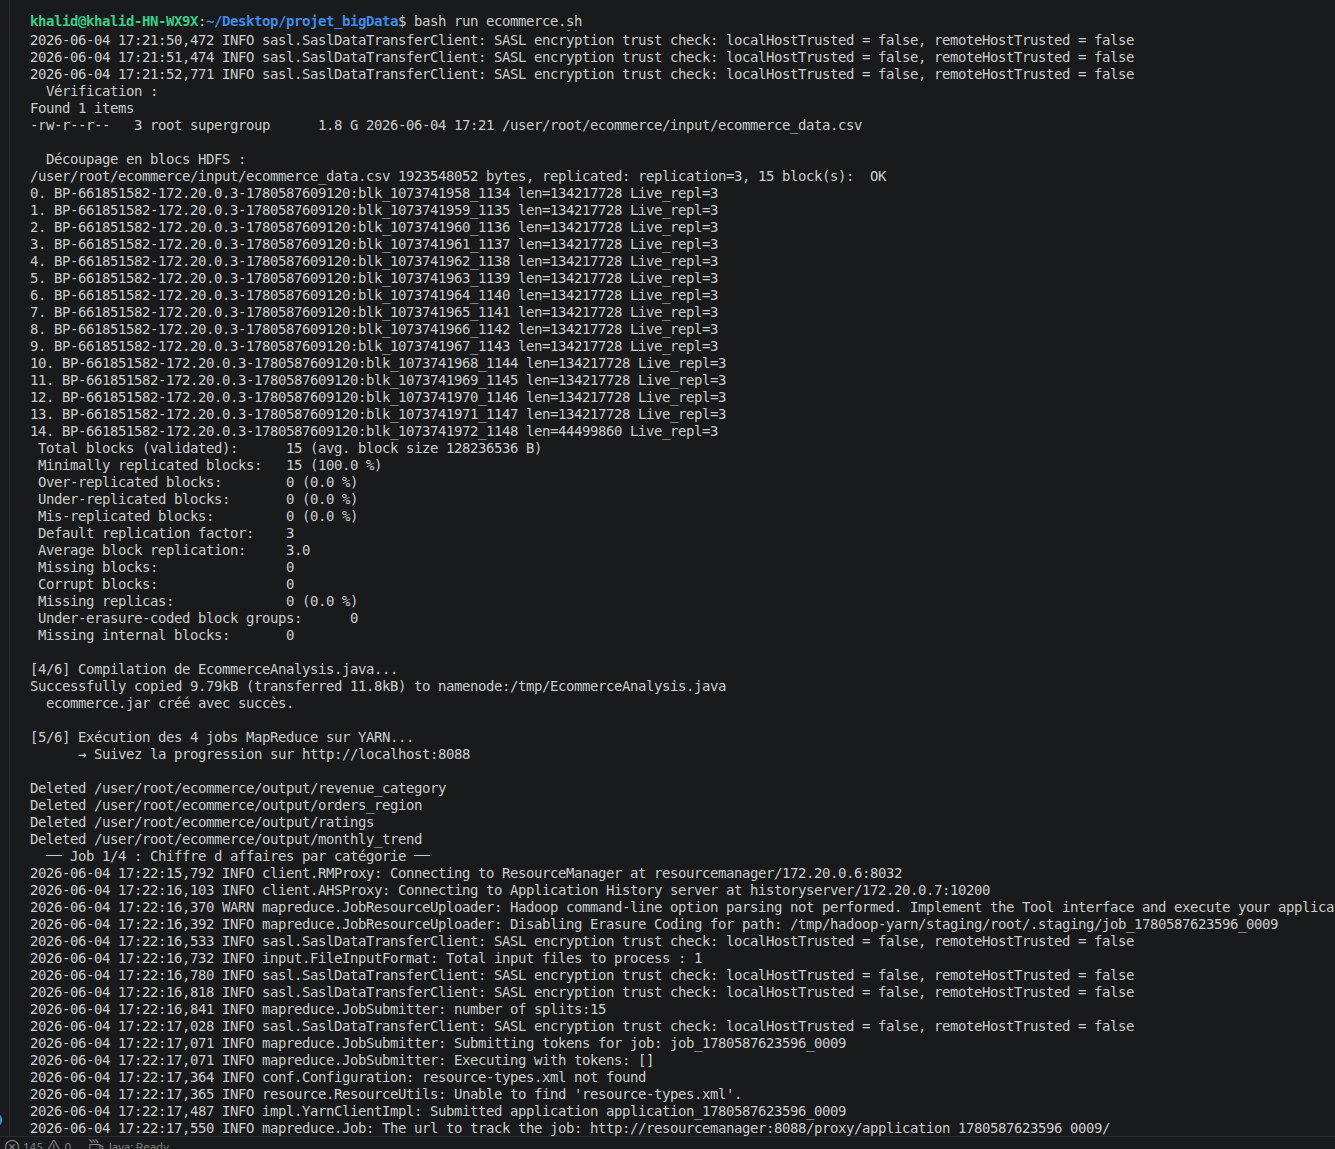
\includegraphics[width=\textwidth]{hdfs_blocs_compilation.png}
  \caption{Vérification des blocs HDFS (15 blocs, réplication=3) et compilation du JAR Java}
  \label{fig:compilation}
\end{figure}

\subsection{Exécution sur YARN — Jobs 1 et 2}

La figure~\ref{fig:job1_exec} montre l'exécution du Job 1
(\textit{revenue\_category}) avec la progression des tâches Map et Reduce.
La figure~\ref{fig:job1_counters} présente les compteurs complets du Job 1
et le démarrage du Job 2 (\textit{orders\_region}).

\begin{figure}[H]
  \centering
  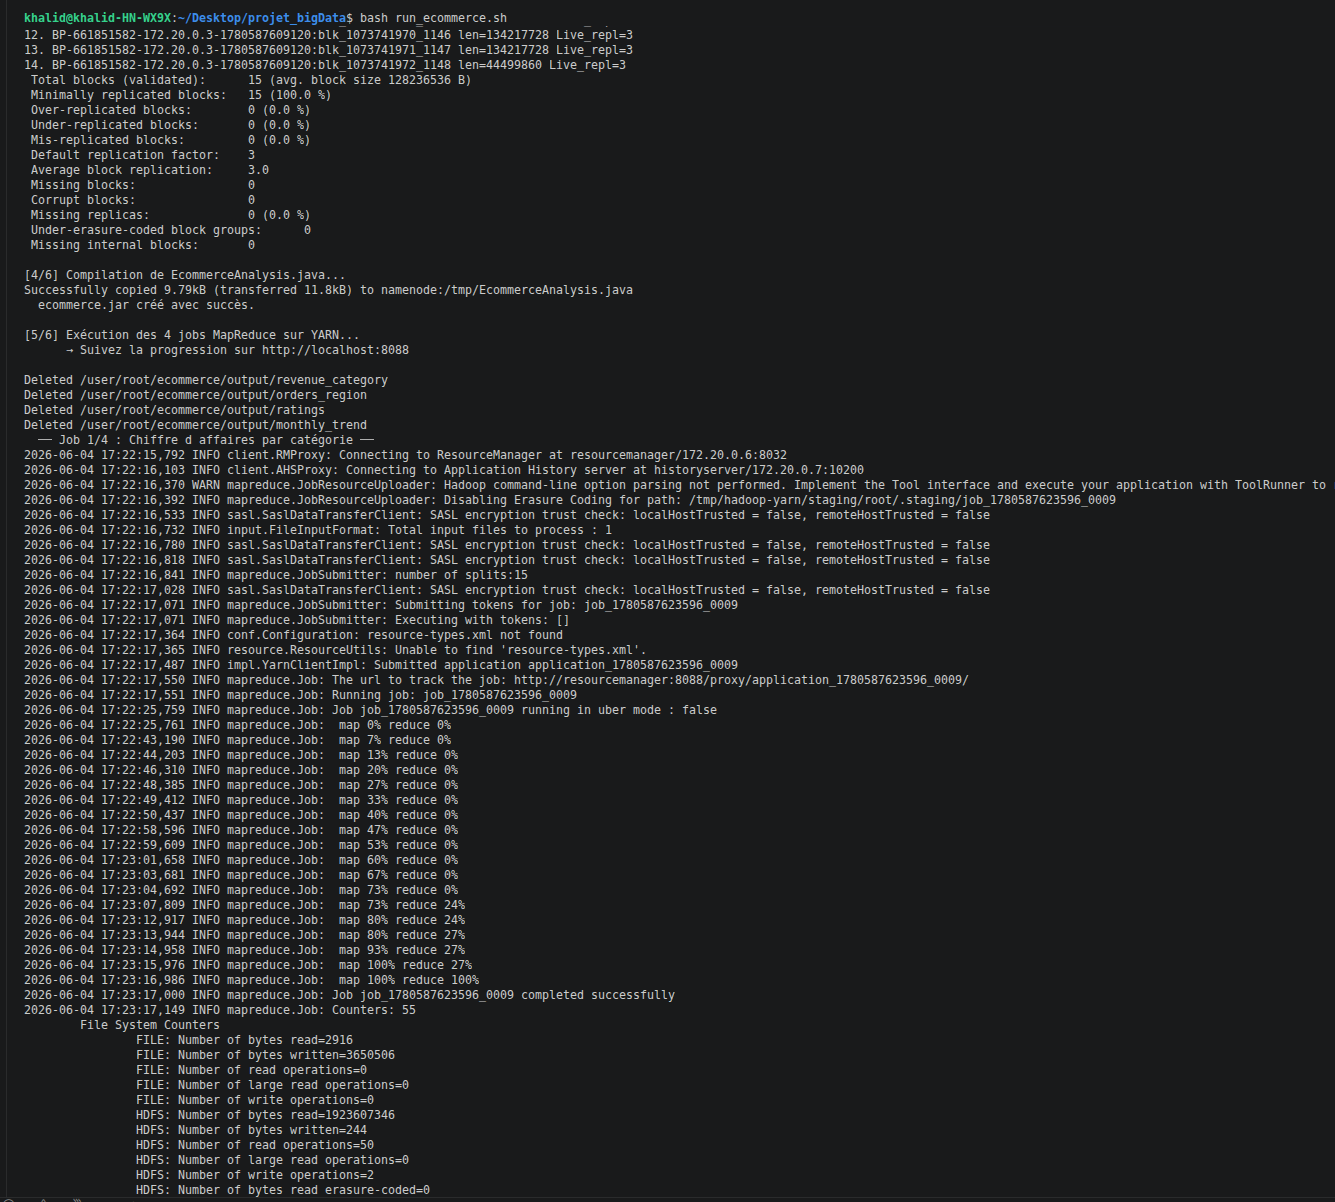
\includegraphics[width=\textwidth]{job1_execution.png}
  \caption{Exécution YARN — Job 1 : \textit{ecommerce-revenue\_category} (Map 100\%, Reduce 100\%)}
  \label{fig:job1_exec}
\end{figure}

\begin{figure}[H]
  \centering
  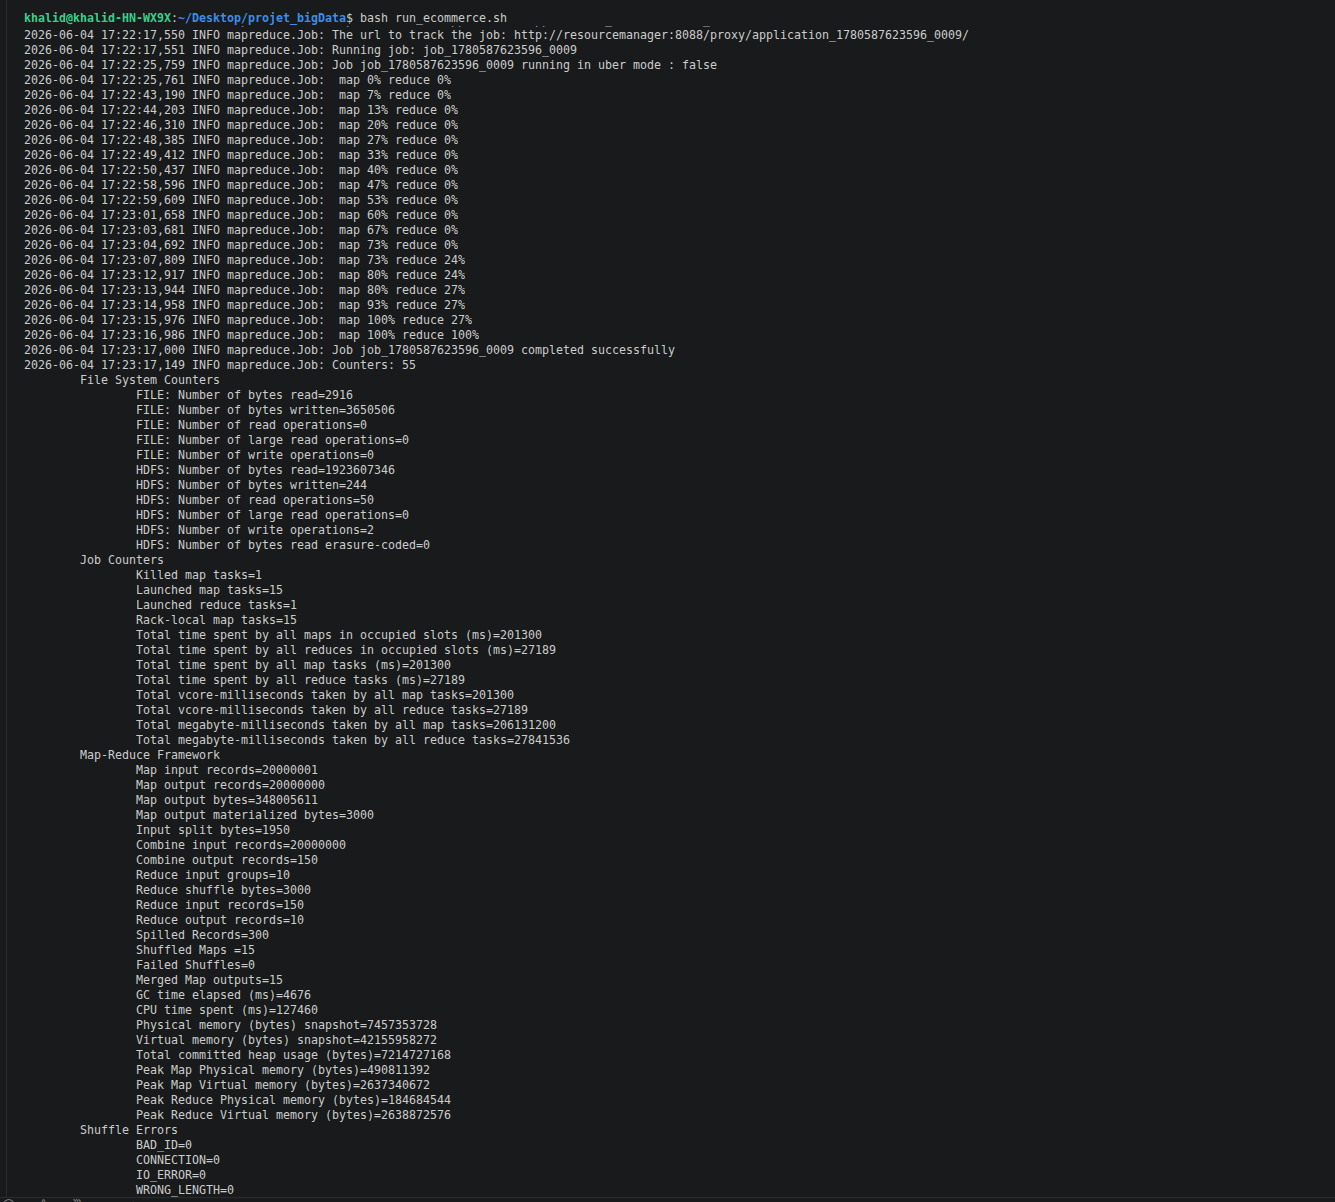
\includegraphics[width=\textwidth]{job1_compteurs_job2.png}
  \caption{Compteurs du Job 1 et lancement du Job 2 (\textit{orders\_region})}
  \label{fig:job1_counters}
\end{figure}

\subsection{Exécution sur YARN — Jobs 2, 3 et 4}

\begin{figure}[H]
  \centering
  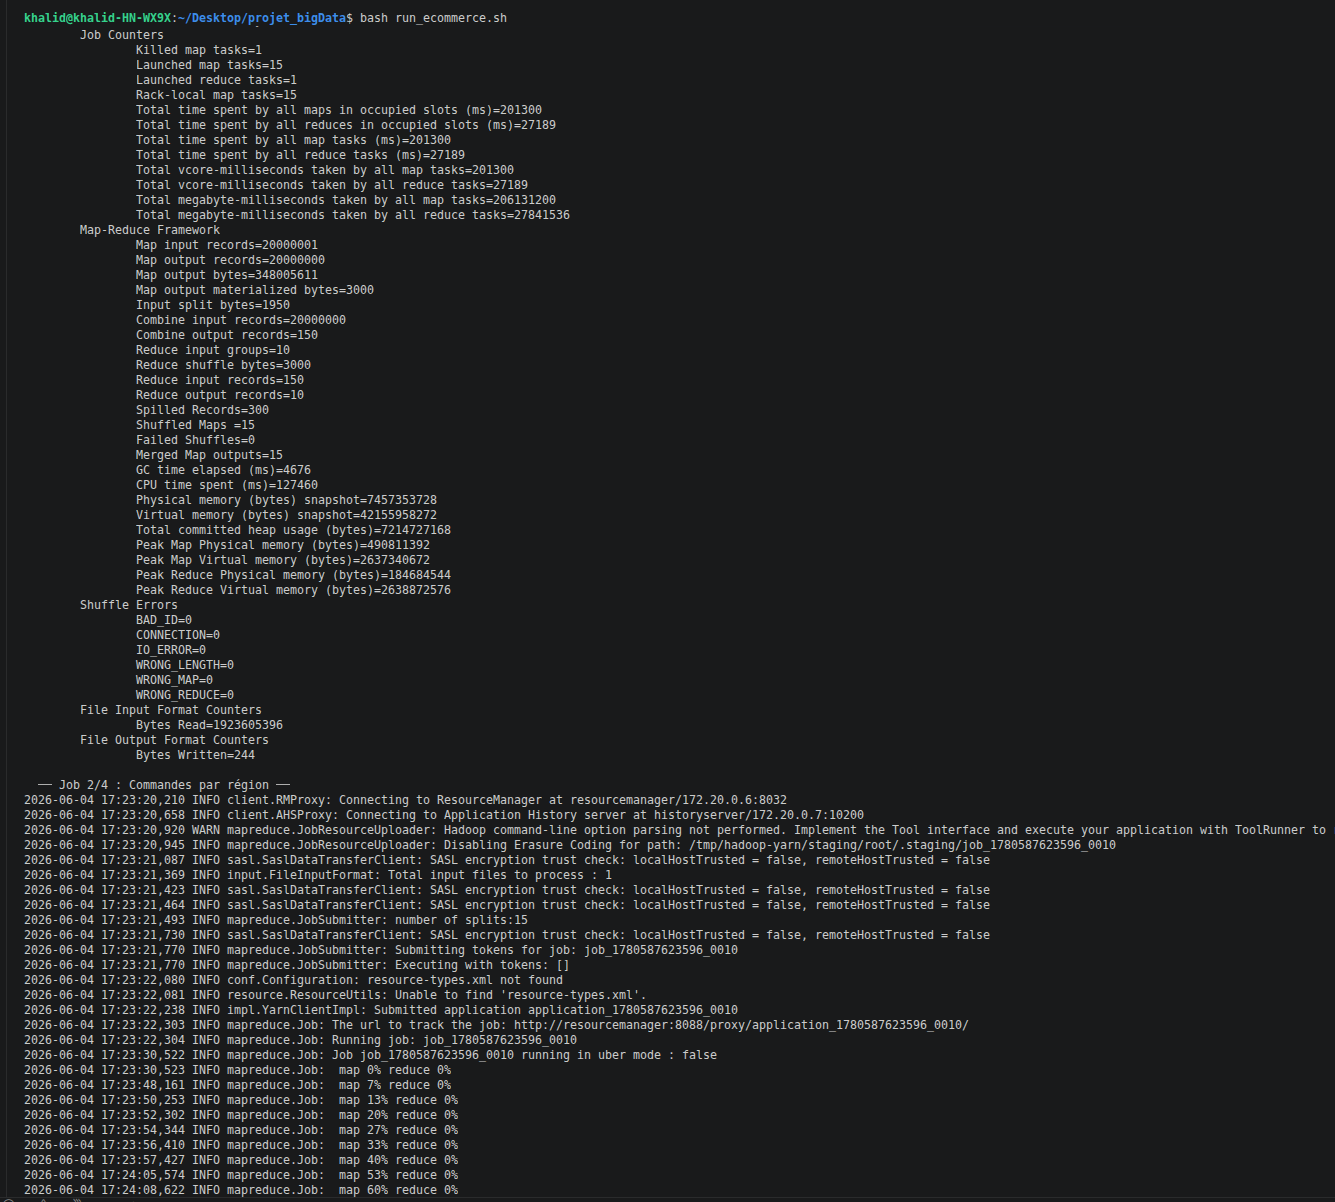
\includegraphics[width=\textwidth]{job2_compteurs_job3.png}
  \caption{Compteurs du Job 2 (\textit{orders\_region}) et lancement du Job 3 (\textit{ratings})}
  \label{fig:job2_job3}
\end{figure}

\begin{figure}[H]
  \centering
  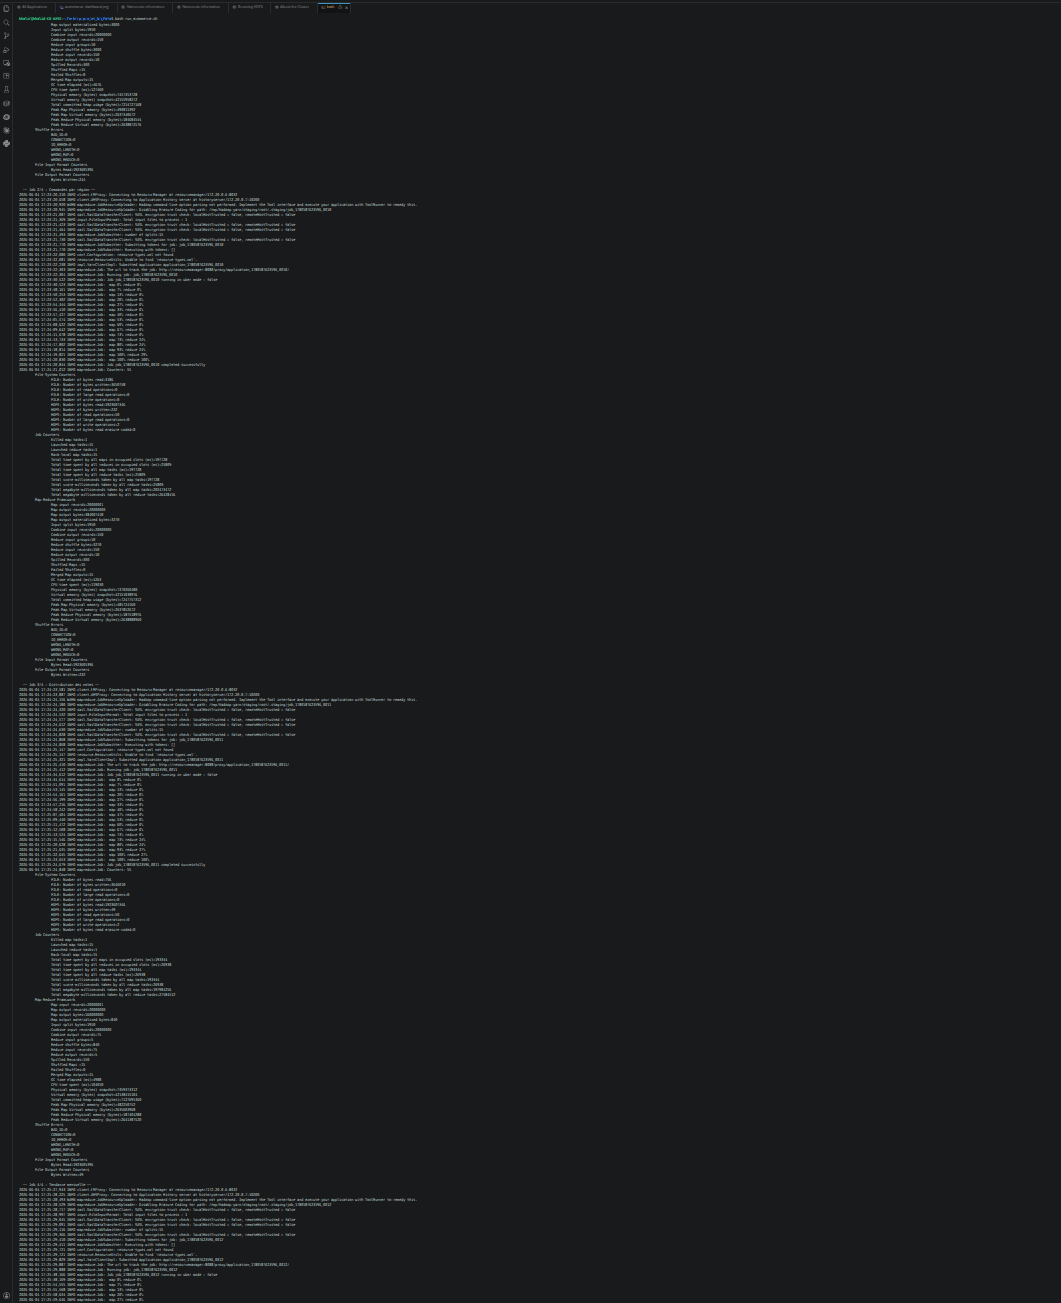
\includegraphics[width=\textwidth]{job3_job4_execution.png}
  \caption{Exécution des Jobs 3 (\textit{ratings}) et 4 (\textit{monthly\_trend})}
  \label{fig:job3_job4}
\end{figure}

\subsection{Interface YARN ResourceManager}

La figure~\ref{fig:yarn} montre l'interface du ResourceManager YARN
(\texttt{localhost:8088}) confirmant que les \textbf{4 applications MapReduce}
ont toutes le statut \textbf{FINISHED / SUCCEEDED}.

\begin{figure}[H]
  \centering
  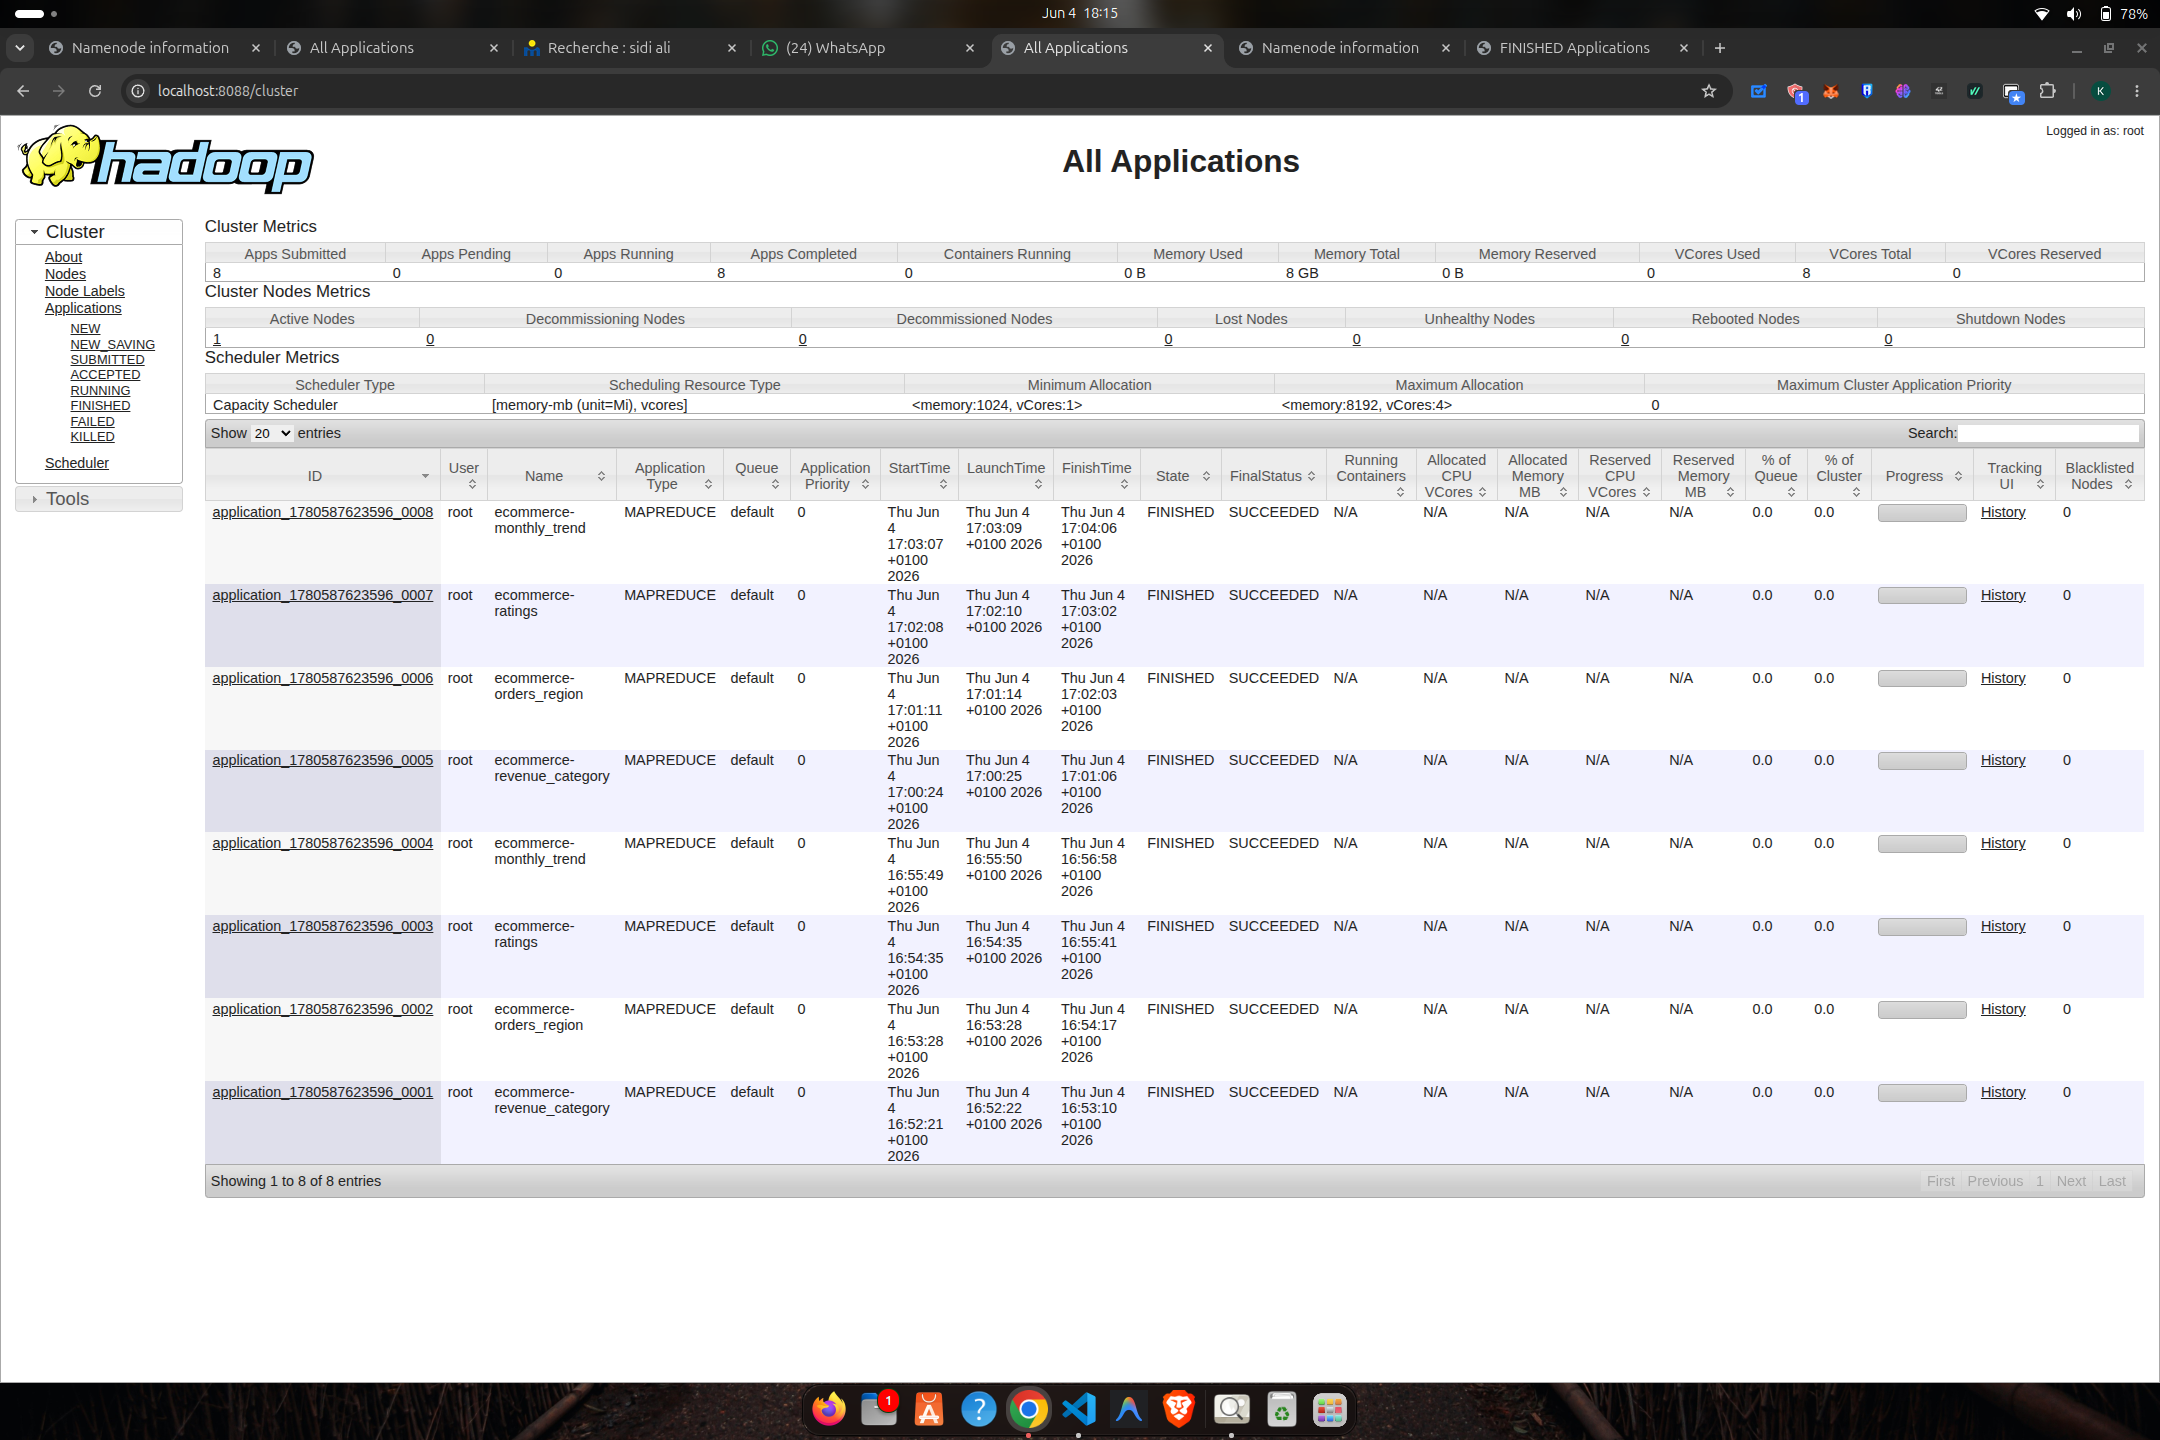
\includegraphics[width=\textwidth]{yarn_applications.png}
  \caption{YARN ResourceManager (\texttt{localhost:8088}) — 4 jobs MapReduce terminés avec succès}
  \label{fig:yarn}
\end{figure}

% ═══════════════════════════════════════════════════════════════════════════════
%  5. RÉSULTATS
% ═══════════════════════════════════════════════════════════════════════════════
\section{Résultats et analyse}
\label{sec:resultats}

\subsection{Résultats affichés par le script}

À la fin de l'exécution, le script \texttt{run\_ecommerce.sh} affiche
automatiquement un tableau récapitulatif de tous les résultats
(figure~\ref{fig:resultats}).

\begin{figure}[H]
  \centering
  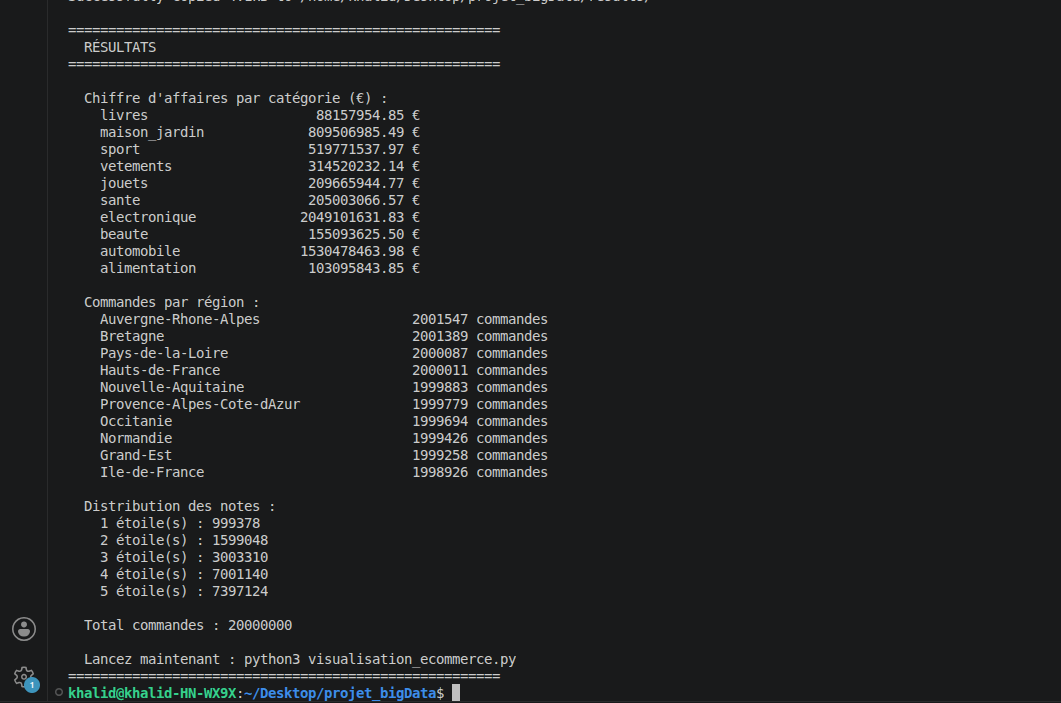
\includegraphics[width=0.9\textwidth]{resultats_finaux.png}
  \caption{Résultats complets affichés par \texttt{run\_ecommerce.sh} —
           CA par catégorie, commandes par région, distribution des notes}
  \label{fig:resultats}
\end{figure}

\subsection{Job 1 — Chiffre d'affaires par catégorie}

\begin{table}[H]
  \centering
  \caption{Chiffre d'affaires par catégorie (sur 20 millions de commandes)}
  \label{tab:ca_categorie}
  \begin{tabular}{lrr}
    \toprule
    \textbf{Catégorie} & \textbf{CA (€)} & \textbf{Part (\%)} \\
    \midrule
    Électronique    & 2\,049\,101\,631 & 37,5 \\
    Automobile      & 1\,530\,478\,463 & 28,0 \\
    Maison/Jardin   & 809\,506\,985    & 14,8 \\
    Sport           & 519\,771\,537    & 9,5  \\
    Vêtements       & 314\,520\,232    & 5,8  \\
    Jouets          & 209\,665\,944    & 3,8  \\
    Santé           & 205\,003\,066    & 3,7  \\
    Beauté          & 155\,093\,625    & 2,8  \\
    Alimentation    & 103\,095\,843    & 1,9  \\
    Livres          & 88\,157\,954     & 1,6  \\
    \midrule
    \textbf{Total}  & \textbf{5\,984\,395\,286} & \textbf{100} \\
    \bottomrule
  \end{tabular}
\end{table}

\textbf{Analyse :} L'électronique domine avec 37,5\% du chiffre d'affaires total,
suivi de l'automobile (28\%). Ces deux catégories représentent plus de 65\% du CA,
ce qui est cohérent avec leurs prix élevés (jusqu'à 2\,000 € et 1\,500 €).
Les livres et l'alimentation, à faible prix unitaire, ne contribuent que
marginalement.

\subsection{Job 2 — Commandes par région}

\begin{table}[H]
  \centering
  \caption{Nombre de commandes par région cliente}
  \label{tab:region}
  \begin{tabular}{lrr}
    \toprule
    \textbf{Région} & \textbf{Commandes} & \textbf{Part (\%)} \\
    \midrule
    Auvergne-Rhône-Alpes       & 2\,001\,547 & 10,01 \\
    Bretagne                   & 2\,001\,389 & 10,01 \\
    Pays-de-la-Loire           & 2\,000\,087 & 10,00 \\
    Hauts-de-France            & 2\,000\,011 & 10,00 \\
    Nouvelle-Aquitaine         & 1\,999\,883 & 10,00 \\
    Provence-Alpes-Côte d'Azur & 1\,999\,779 & 10,00 \\
    Occitanie                  & 1\,999\,694 & 10,00 \\
    Normandie                  & 1\,999\,426 & 10,00 \\
    Grand-Est                  & 1\,999\,258 & 9,99  \\
    Île-de-France              & 1\,998\,926 & 9,99  \\
    \midrule
    \textbf{Total}             & \textbf{20\,000\,000} & \textbf{100} \\
    \bottomrule
  \end{tabular}
\end{table}

\textbf{Analyse :} La distribution est quasi-uniforme ($\approx$2 millions par région),
conformément au processus de génération aléatoire uniforme. Dans un contexte réel,
l'Île-de-France représenterait une part bien plus importante en raison de sa densité
de population.

\subsection{Job 3 — Distribution des notes clients}

\begin{table}[H]
  \centering
  \caption{Distribution des évaluations clients}
  \label{tab:ratings}
  \begin{tabular}{lcrrr}
    \toprule
    \textbf{Note} & \textbf{Étoiles} & \textbf{Nombre} & \textbf{Part (\%)} & \textbf{Poids générat.} \\
    \midrule
    1 & ★☆☆☆☆ & 999\,378    & 5,0  & 5  \\
    2 & ★★☆☆☆ & 1\,599\,048 & 8,0  & 8  \\
    3 & ★★★☆☆ & 3\,003\,310 & 15,0 & 15 \\
    4 & ★★★★☆ & 7\,001\,140 & 35,0 & 35 \\
    5 & ★★★★★ & 7\,397\,124 & 37,0 & 37 \\
    \midrule
    \textbf{Total} & & \textbf{20\,000\,000} & \textbf{100} & \\
    \bottomrule
  \end{tabular}
\end{table}

\textbf{Calcul de la note moyenne :}
\[
\bar{x} = \frac{1 \times 999\,378 + 2 \times 1\,599\,048 + 3 \times 3\,003\,310
               + 4 \times 7\,001\,140 + 5 \times 7\,397\,124}{20\,000\,000}
        \approx \mathbf{3{,}96\ / \ 5}
\]

\textbf{Analyse :} La distribution skew-positive (72\% de notes 4 ou 5 étoiles)
reflète fidèlement le comportement observé sur les plateformes e-commerce réelles.

\subsection{Job 4 — Tendance mensuelle}

\begin{table}[H]
  \centering
  \caption{Chiffre d'affaires mensuel — échantillon (48 mois)}
  \label{tab:monthly}
  \begin{tabular}{lrlr}
    \toprule
    \textbf{Mois} & \textbf{CA (M€)} & \textbf{Mois} & \textbf{CA (M€)} \\
    \midrule
    2020-01 & 127,4 & 2022-01 & 127,2 \\
    2020-06 & 122,8 & 2022-06 & 123,2 \\
    2020-12 & 127,2 & 2022-12 & 127,1 \\
    2021-01 & 126,4 & 2023-01 & 126,5 \\
    2021-06 & 122,9 & 2023-06 & 122,9 \\
    2021-12 & 126,9 & 2023-12 & 122,9 \\
    \bottomrule
  \end{tabular}
\end{table}

\textbf{Analyse :} Le CA mensuel oscille régulièrement entre 122 M€ (mois courts)
et 127 M€ (mois longs). La stabilité reflète la distribution aléatoire uniforme
du dataset synthétique. Une légère saisonnalité est perceptible avec des CA plus
faibles en février.

% ═══════════════════════════════════════════════════════════════════════════════
%  6. VISUALISATION
% ═══════════════════════════════════════════════════════════════════════════════
\section{Visualisation — Dashboard}
\label{sec:visu}

\subsection{Sortie du script de visualisation}

Le script Python \texttt{visualisation\_ecommerce.py} lit les quatre fichiers
de résultats MapReduce, calcule les statistiques globales et génère un dashboard.
La figure~\ref{fig:python_output} montre sa sortie console.

\begin{figure}[H]
  \centering
  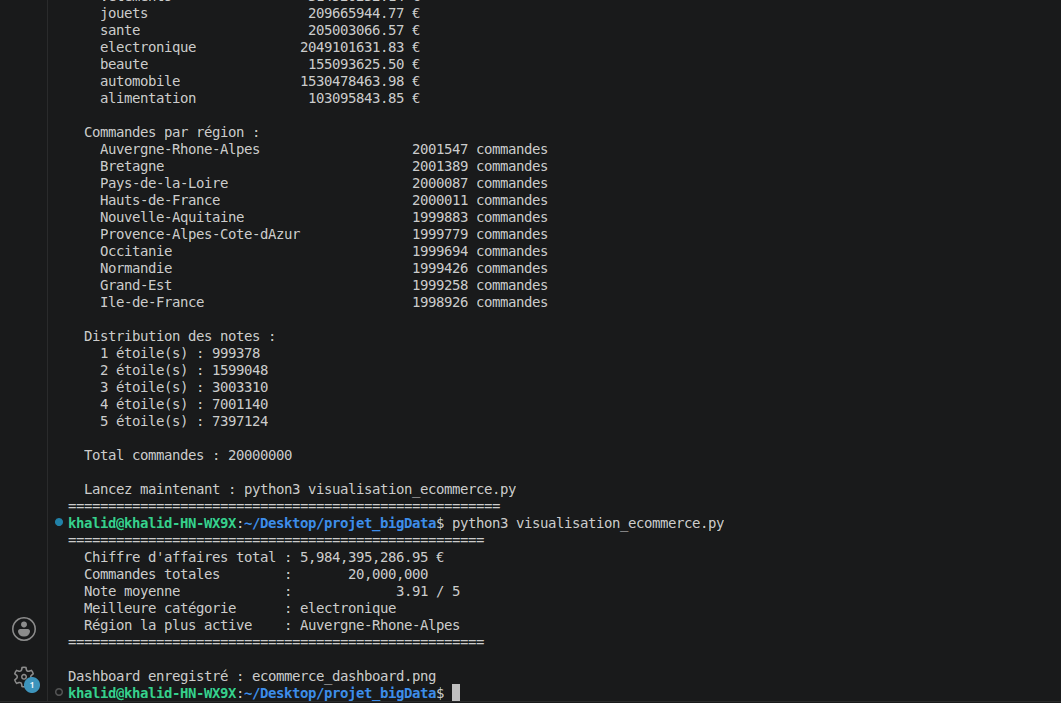
\includegraphics[width=0.85\textwidth]{python_dashboard_output.png}
  \caption{Sortie de \texttt{python3 visualisation\_ecommerce.py} — statistiques globales
           et confirmation de génération du dashboard}
  \label{fig:python_output}
\end{figure}

\begin{tcolorbox}[colback=accentGreen!8, colframe=accentGreen,
                  title=Statistiques globales calculées par le script Python]
  \begin{tabular}{ll}
    Chiffre d'affaires total & 5\,984\,395\,286,95 € ($\approx$ 5,98 milliards) \\
    Commandes totales        & 20\,000\,000 \\
    Note moyenne             & 3,91 / 5 \\
    Meilleure catégorie CA   & Électronique \\
    Région la plus active    & Auvergne-Rhône-Alpes \\
  \end{tabular}
\end{tcolorbox}

\subsection{Dashboard généré}

Le dashboard (figure~\ref{fig:dashboard}) présente en 2×2 graphiques :
\begin{enumerate}
  \item \textbf{Haut gauche :} CA par catégorie en barres horizontales (M€, ordre décroissant).
  \item \textbf{Haut droite :} Commandes par région en barres horizontales.
  \item \textbf{Bas gauche :} Histogramme coloré des notes (rouge pour 1★, vert pour 5★).
  \item \textbf{Bas droite :} Courbe de tendance mensuelle du CA (2020--2023).
\end{enumerate}

\begin{figure}[H]
  \centering
  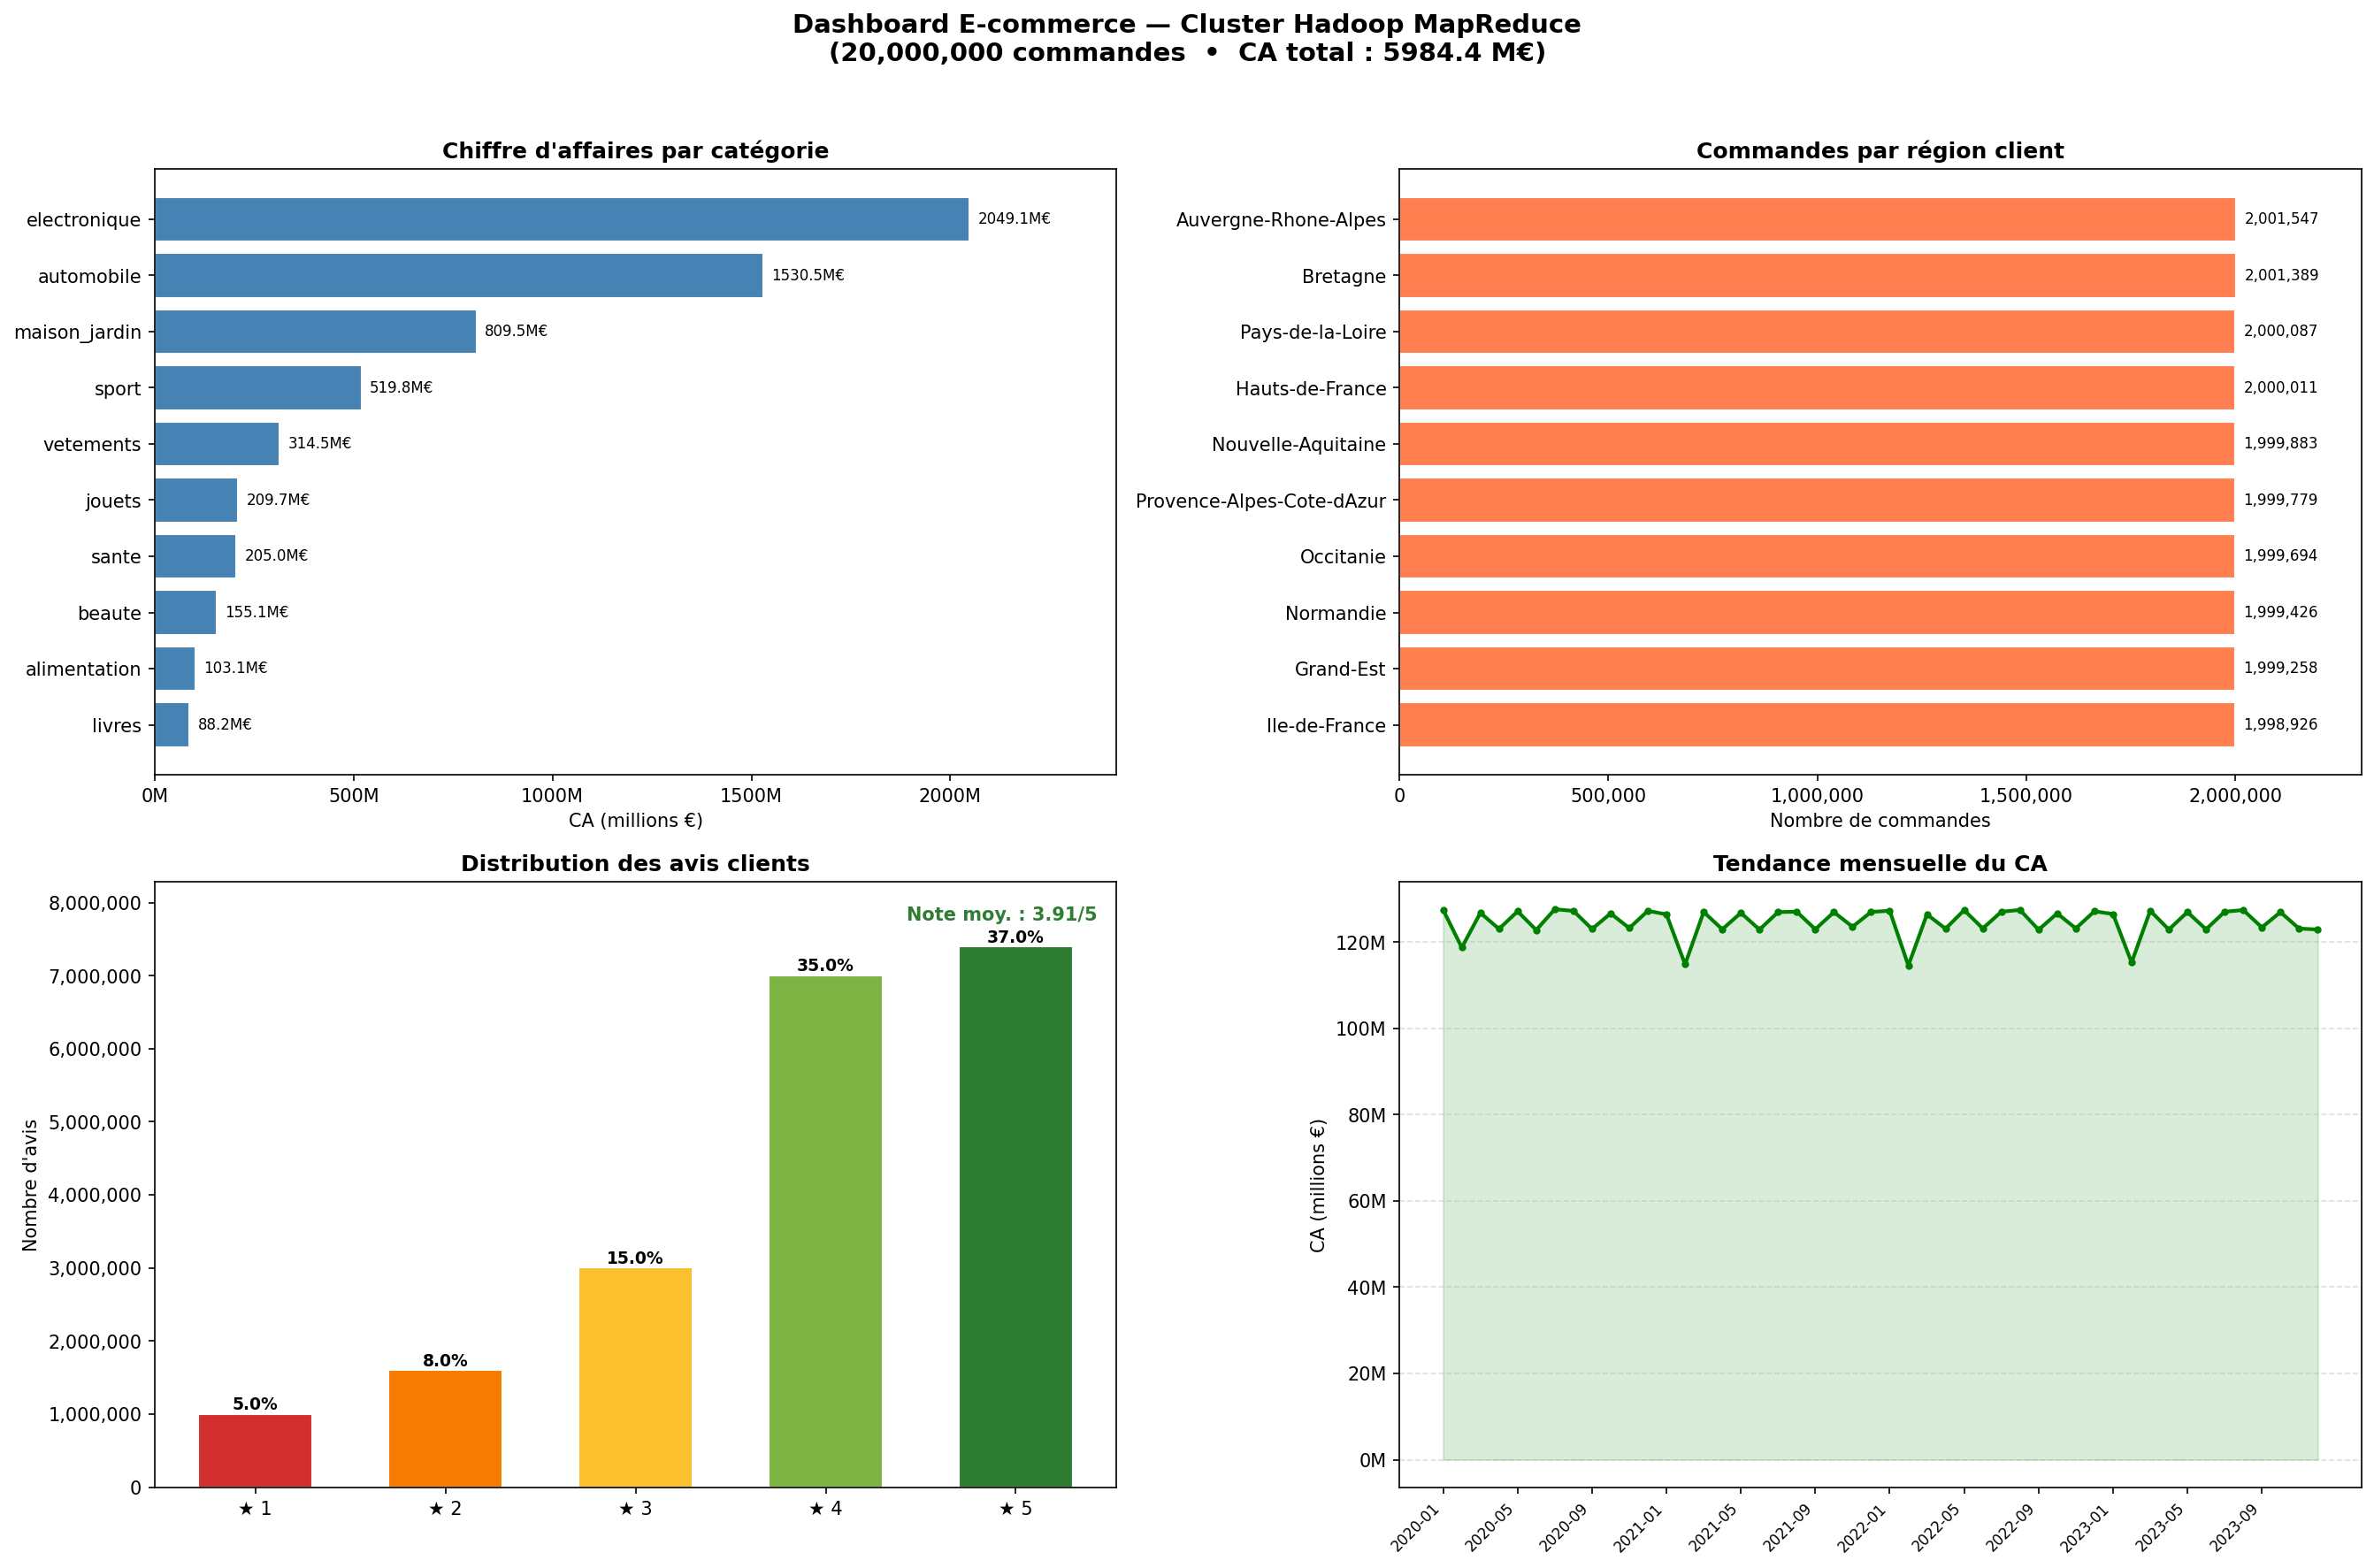
\includegraphics[width=\textwidth]{dashboard.png}
  \caption{Dashboard e-commerce — 20 millions de commandes analysées par Hadoop MapReduce}
  \label{fig:dashboard}
\end{figure}

% ═══════════════════════════════════════════════════════════════════════════════
%  7. CONCLUSION
% ═══════════════════════════════════════════════════════════════════════════════
\section{Conclusion}
\label{sec:conclusion}

\subsection{Bilan du projet}

Ce projet a permis de mettre en œuvre l'ensemble du cycle de traitement Big Data :

\begin{itemize}
  \item \textbf{Infrastructure} : déploiement d'un cluster Hadoop distribué à
        7 nœuds via Docker Compose, avec HDFS (réplication 3) et YARN.
  \item \textbf{Données} : génération d'un dataset synthétique e-commerce
        réaliste de 20 millions de lignes (1,8 Go), découpé en 15 blocs HDFS.
  \item \textbf{Traitement} : implémentation de quatre jobs MapReduce en Java,
        chacun adressant une problématique analytique distincte.
  \item \textbf{Optimisation} : utilisation systématique du Combiner pour
        réduire le trafic réseau lors du shuffle.
  \item \textbf{Résultats} : les 4 jobs YARN se sont tous terminés avec le
        statut \texttt{FINISHED / SUCCEEDED}, traitant 20 millions de lignes.
  \item \textbf{Visualisation} : production d'un dashboard matplotlib
        synthétisant les quatre analyses en un seul graphique.
\end{itemize}

\subsection{Limites et perspectives}

\begin{itemize}
  \item Le cluster tourne en local sur une seule machine physique ; les gains
        de performance distribués ne sont pas pleinement exploités.
  \item Les jobs sont exécutés séquentiellement ; une orchestration avec
        \textbf{Apache Oozie} permettrait leur parallélisation.
  \item L'introduction d'\textbf{Apache Hive} ou de \textbf{Apache Spark SQL}
        simplifierait les requêtes analytiques par rapport au MapReduce natif.
  \item Le dataset synthétique pourrait être remplacé par des données réelles
        (ex. : dataset Olist Brazil disponible sur Kaggle).
\end{itemize}

\subsection{Compétences acquises}

Ce projet a permis d'acquérir une maîtrise pratique de : l'administration d'un
cluster Hadoop, la programmation du paradigme MapReduce en Java, la gestion de
HDFS en ligne de commande, la conteneurisation Docker pour les systèmes
distribués, et la visualisation de données volumineuses avec Python/Matplotlib.

% ═══════════════════════════════════════════════════════════════════════════════
%  ANNEXES
% ═══════════════════════════════════════════════════════════════════════════════
\appendix

\section{Structure complète du projet}

\begin{lstlisting}[caption={Arborescence des fichiers du projet}]
projet_bigData/
├── docker-compose.yml          # Definition du cluster (7 services)
├── hadoop.env                  # Variables d'environnement Hadoop
├── generate_dataset.py         # Generateur du dataset (20 M lignes)
├── EcommerceAnalysis.java      # 4 jobs MapReduce (Java)
├── visualisation_ecommerce.py  # Dashboard matplotlib
├── run_ecommerce.sh            # Script d'orchestration complet
├── ecommerce_data.csv          # Dataset genere (1,8 Go)
├── ecommerce_dashboard.png     # Dashboard PNG genere
├── images_Rapport/             # Screenshots pour le rapport
└── results/
    ├── revenue_category/part-r-00000
    ├── orders_region/part-r-00000
    ├── ratings/part-r-00000
    └── monthly_trend/part-r-00000
\end{lstlisting}

\section{Résultats bruts MapReduce}

\subsection*{revenue\_category/part-r-00000}
\begin{lstlisting}
alimentation    1.0309584385E8
automobile      1.53047846398E9
beaute          1.550936255E8
electronique    2.04910163183E9
jouets          2.0966594477E8
livres          8.815795485E7
maison_jardin   8.0950698549E8
sante           2.0500306657E8
sport           5.1977153797E8
vetements       3.1452023214E8
\end{lstlisting}

\subsection*{orders\_region/part-r-00000}
\begin{lstlisting}
Auvergne-Rhone-Alpes        2001547
Bretagne                    2001389
Grand-Est                   1999258
Hauts-de-France             2000011
Ile-de-France               1998926
Normandie                   1999426
Nouvelle-Aquitaine          1999883
Occitanie                   1999694
Pays-de-la-Loire            2000087
Provence-Alpes-Cote-dAzur   1999779
\end{lstlisting}

\subsection*{ratings/part-r-00000}
\begin{lstlisting}
1   999378
2   1599048
3   3003310
4   7001140
5   7397124
\end{lstlisting}

\end{document}
